\documentclass{article}


\usepackage{arxiv}

\usepackage[utf8]{inputenc} % allow utf-8 input
\usepackage[T1]{fontenc}    % use 8-bit T1 fonts
\usepackage[hyphens]{url}
\usepackage{hyperref}       % hyperlinks
\usepackage{booktabs}       % professional-quality tables
\usepackage{amsfonts}       % blackboard math symbols
\usepackage{nicefrac}       % compact symbols for 1/2, etc.
\usepackage{microtype}      % microtypography
\usepackage{lipsum}
\usepackage{graphicx}
\usepackage{caption}
\captionsetup[table]{skip=10pt}
\usepackage{amsmath}
\usepackage{wrapfig}
\usepackage{siunitx}
\usepackage{float}
\usepackage{booktabs}
\usepackage{multirow}
%\usepackage{refcheck}

\graphicspath{ {./images/} }


\title{Point cloud classification using deep neural networks}

\author{
 Federica Di Lauro \\
  829470\\
  \texttt{f.dilauro2@campus.unimib.it} \\
   \And
  Andrea Premate \\
  829777\\
  \texttt{a.premate@campus.unimib.it} \\
  \And
  Lidia Lucrezia Tonelli \\
  813114\\
  \texttt{l.tonelli@campus.unimib.it} \\
}

\begin{document}
\maketitle
\begin{abstract}
Point clouds are a particular type of data, made of an unordered list of 3D points in space. Feeding a deep neural network with this type of input, for tasks such as classification, segmentation and so on, is not a trivial task because there is no intrinsic geometric structure in the data, but the geometric structure of the point cloud is fundamental to extract information. In this in-depth study we analyze multiple approaches that have been proposed in literature. We limit our study to the classification task, since it's the task that have been first treated in literature and the neural network developed for it are used as backbones for more difficult tasks.
\end{abstract}

\section{Introduction}\label{sec:intro}

3D data acquired by sensors such as LiDARs and RGB-D (RGB point and depth value) cameras, complemented with 2D images, can make machines able to understand the surrounding environment; these data have rich geometric, shape and scale information and therefore have several areas of application, including autonomous driving, robotics, remote sensing and medical treatment~\cite{guo2020deep}.

Point cloud understanding includes many tasks, some of which are fundamental tasks in images, such as \textbf{classification}, that aims to assign to each object in the scene a category or class, \textbf{segmentation}, that is the task of labeling each individual point (it can be semantic or instance), and \textbf{object detection}, a recent research topic which objective is to locate all the objects in a given scene. Other tasks in point cloud are tracking (estimating the location of an instance in subsequent frames), flow estimation (estimating the flow among sequences of point clouds), matching and registration (finding the relationship between point clouds of the same scene collected in different ways), augmentation and completion (improving the quality of raw point clouds), and reconstruction.

In this survey some of the main existent approaches to point cloud classification will be described.

\paragraph{Point Cloud}

A point cloud is a set of data points in space that may represent a 3D shape or object; each point is identified by a set of Cartesian coordinates $(x,y,z)$. 3D scanners or photogrammetry software produce sets of data by measuring many points on the surfaces of objects in their surrounding environment.

3D data can have different formats: depth images, point clouds, meshes and volumetric grids; point clouds representation is a very used format because it preserves the geometric information without discretization. In contrast to image data, point clouds don't directly contain intrinsic spatial structure because they're composed by a set of 3D coordinates and they're not arranged in an array like images.

Deep learning techniques have recently been used to face many tasks in computer vision, especially image tasks; because of the difference between an image task and a 3D point cloud task, in order to apply deep learning to this type of data there are three main problems to be solved: find a dense representation from a sparse point cloud, build a network satisfying size-variance and permutation-invariance restrictions, process large volumes of data in lower time and computational resources~\cite{lu2020deep}.

% A general taxonomy of deep learning methods for 3D point clouds is illustrated in \ref{fig:taxonomy_point_clouds}: tasks can be divided in the three categories of classification, segmentation, and detection and tracking.

% \begin{figure}[ht]
%     \centering
%     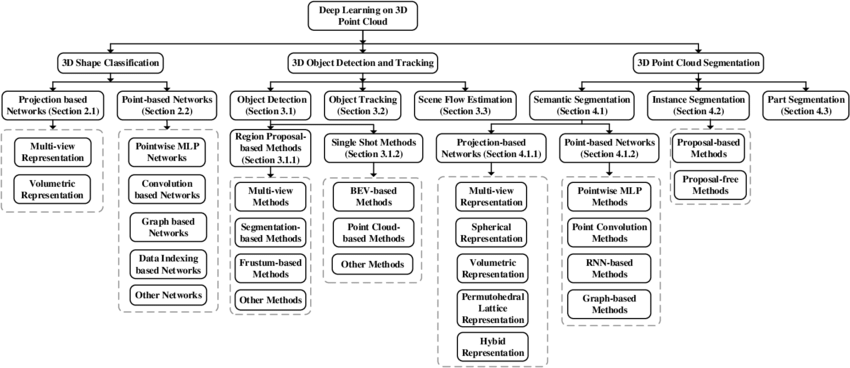
\includegraphics[width=0.85\textwidth]{images/taxonomy_point_clouds.png}
%     \caption{A taxonomy of deep learning methods for 3D point clouds.}
%     \label{fig:taxonomy_point_clouds}
% \end{figure}

\paragraph{Classification task}

In this survey we will describe the task of classification on point clouds, since it's the first task to have been treated in the literature. Classification on point clouds is known as 3D shape classification and it's similar to image classification: methods usually learn the embedding of each point in the point cloud, then extract a global shape embedding for the whole cloud with an aggregation encoder; the global embedding is passed through fully connected layers to obtain the expected class. Classification models can be divided in projection-based methods and point-based methods, that will be illustrated in the next sections. Some important classification models in chronological order are shown in figure~\ref{fig:chrono_deep} (\cite{guo2020deep}).

\begin{figure}[ht]
    \centering
    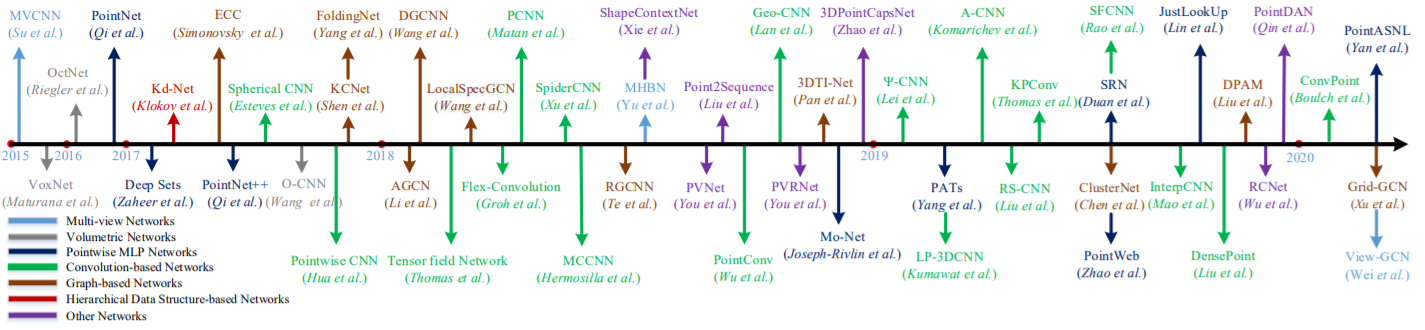
\includegraphics[width=\textwidth]{images/chrono_deep.png}
    \caption{Relevant deep learning models for point cloud classification~\cite{guo2020deep}.}
    \label{fig:chrono_deep}
\end{figure}

\subsection{Datasets}
\label{subsec:datasets}

Well-designed datasets are needed to evaluate the performances of deep learning algorithms on 3D point clouds applications and help defining new tasks and research topics on the subject. 3D datasets are usually small because their capture requires much more effort than 2D images, and efficiently providing dense annotations in 3D is non-trivial~\cite{dai2017scannet}.

For the task of classification, datasets can be synthetic or real-world: the former are complete and don't have occlusions and background, the latter are occluded at different levels and some objects are contaminated with background noise. 
% For the tasks of detection and tracking, datasets can be indoor scenes or outdoor urban scenes (used for autonomous driving).

\subsubsection{Synthetic datasets}

\paragraph{ModelNet40~\cite{ShapeNets}}
\label{ModNet40}
ModelNet is a large-scale object dataset of 3D computer graphics CAD models, constructed initially to train a 3D deep learning model called 3D ShapeNets. ModelNet is constructed from downloaded 3D CAD models labelled first with Amazon Mechanical Turk and then manually checked. It contains 151,128 3D CAD models belonging to 660 unique object categories. 

ModelNet project provides three benchmarks: ModelNet10, ModelNet40 and Aligned40 (where the numbers stand for the number of categories). 

% Examples of classes and models of ModelNet40 are shown in figure \ref{fig:modelnet}.

This dataset, along with ShapeNet, is often used to evaluate the capacity of backbones before applying it to more complicated tasks. Since ModelNet40 is composed of CAD models and not point clouds, to use the points coordinates as input in the developed networks, the CAD models are sampled to reproduce point clouds. For example, to evaluate classification with PointNet, described later in section~\ref{par:pointnet}, 1024 points are sampled uniformly from the mesh faces of the CAD models, an example is shown in image~\ref{fig:modelnet_sampled}, while figure~\ref{fig:modelnet} shows examples of classes and models present in ModelNet40.

\begin{figure}[hbt]
    \centering
    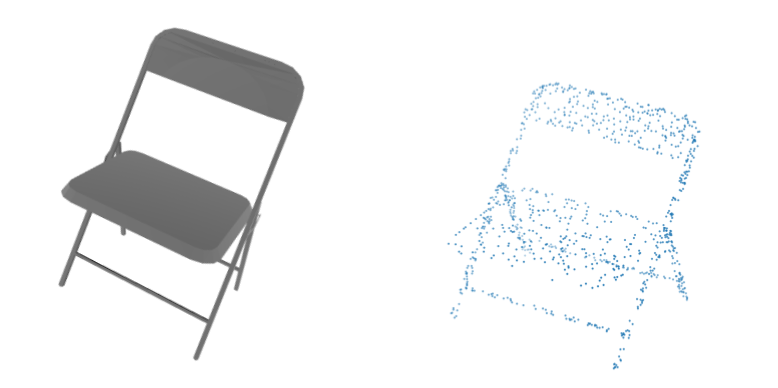
\includegraphics[width=0.6\textwidth]{images/cad_pointcloud.png}
    \caption{Left: CAD model from ModelNet40. Right: point cloud sampled randomly from the CAD model, 1024 points used.}
    \label{fig:modelnet_sampled}
\end{figure}

\begin{figure}[ht]
    \centering
    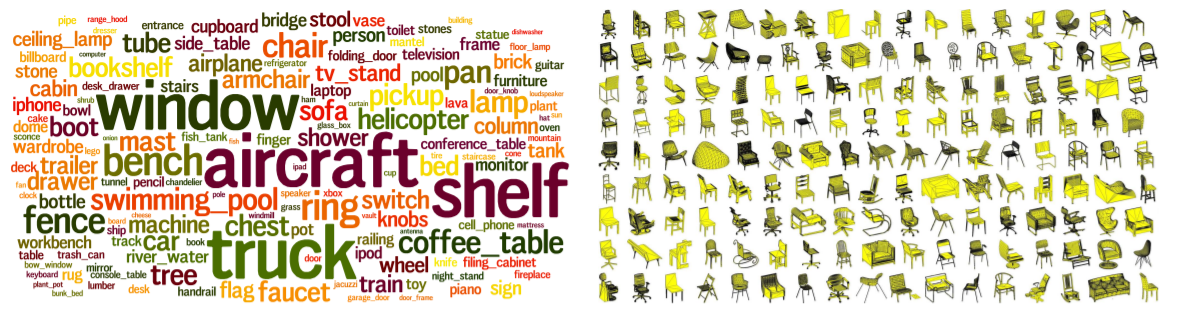
\includegraphics[width=1\textwidth]{images/modelnet.png}
    \caption{ModelNet40. Left: word cloud visualization of the ModelNet dataset. Right: examples of 3D chair models~\cite{ShapeNets}.}
    \label{fig:modelnet}
\end{figure}

\paragraph{ShapeNet~\cite{chang2015shapenet}}

ShapeNet is a repository of shapes represented by 3D CAD models for object of the everyday world, therefore it is a synthetic dataset of point clouds. It is richly-annotation and contains models spanning a multitude of semantic categories: there are 55 categories and they are organized in a hierarchical way according to WordNet synets ("synonym sets"). ShapeNet has a rich set of annotation for each shape and correspondences between them, the annotations are geometric attributes such as orientation vectors, parts and keypoints, shape symmetries and scale of object in real world units.

% The 3D model data comes from online repositories or existing research datasets, ShapeNet is intended to be an evolving dataset with regular updates. The objects are from the everyday world, so there are no CAD mechanical parts, molecular structures nor domain-specific objects. Figure \ref{fig:shapenet} shows some models from ShapeNet.

% \begin{figure}[ht]
%     \centering
%     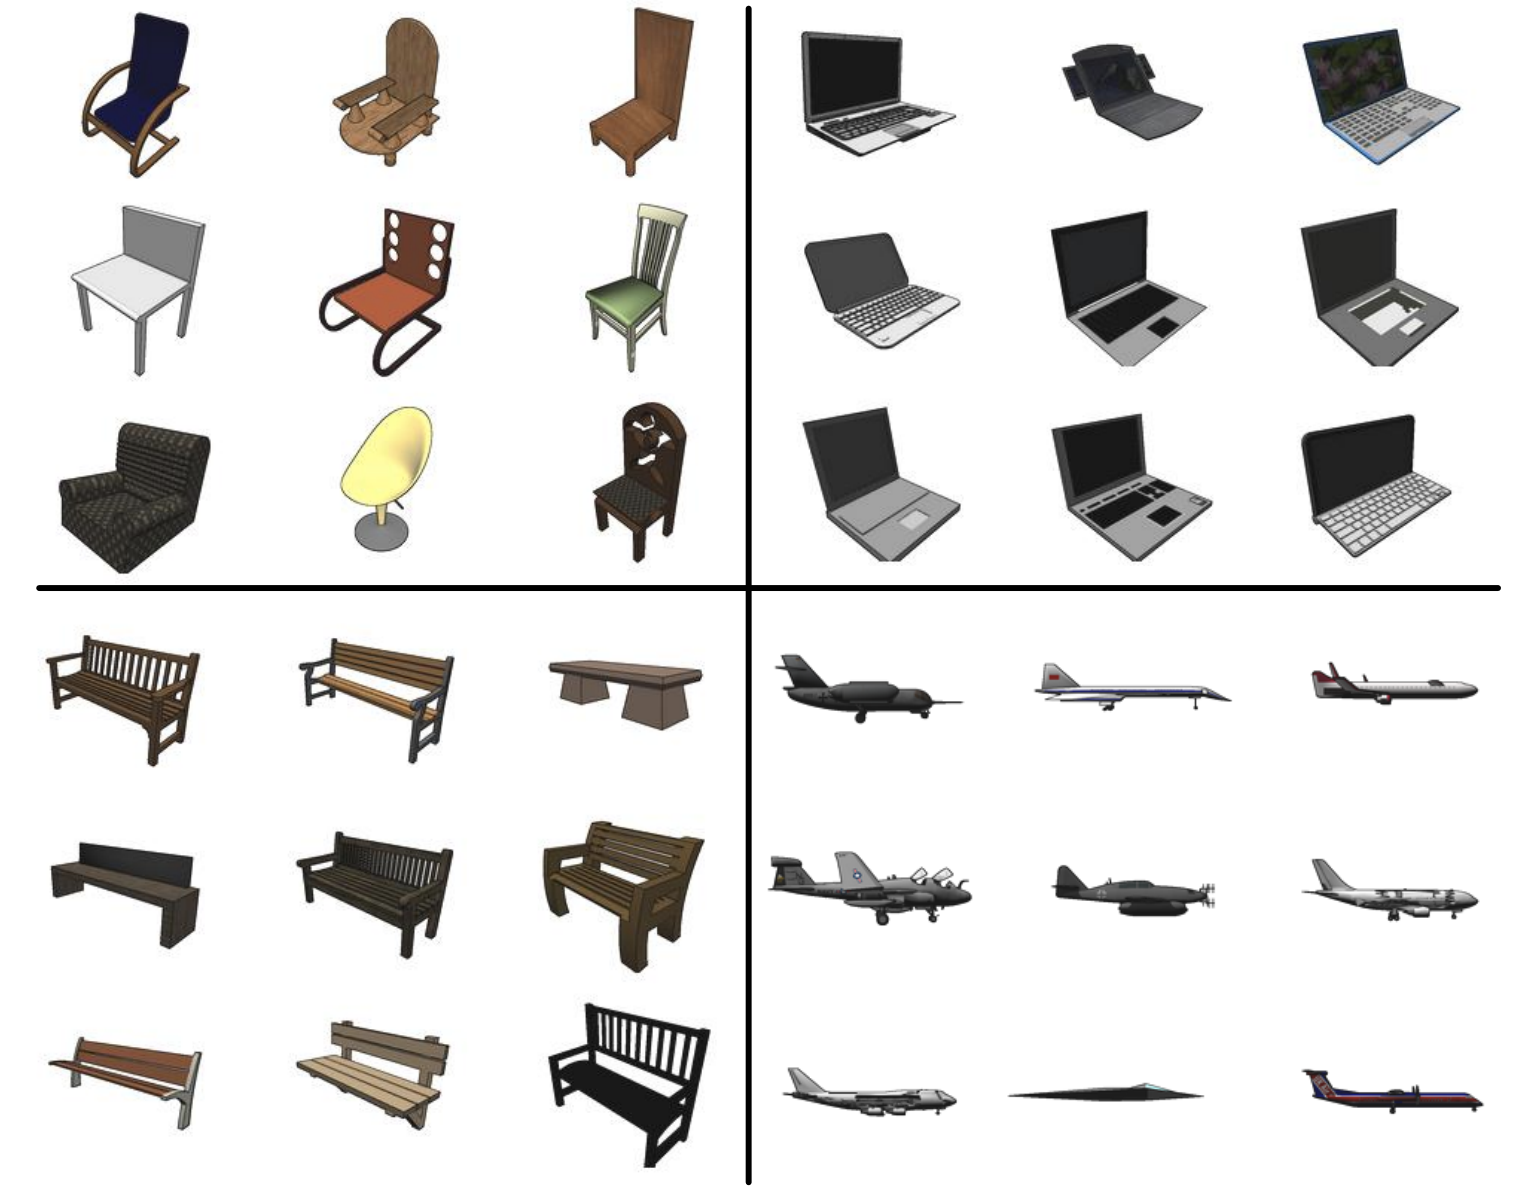
\includegraphics[width=0.5\textwidth]{images/shapenet.png}
%     \caption{Some models of everyday world objects from the ShapeNet Dataset.}
%     \label{fig:shapenet}
% \end{figure}

% The annotations in ShapeNet contain semantic information about the models, establish links between them and link to other modalities of data, such as images. There are different types of annotations: language-related annotations are synets from WorldNet taxonomy and they permit to name objects, for the aims of indexing, grouping and linking to related sources of data; geometric annotations represent objects from the structural point of view, they consist of rigid alignments, parts and keypoints, symmetries, and sizes; functional annotations describe the usage of represented objects, they are usually highly correlated with specific regions of an object, so they can include functional parts or affordances; physical annotations refer to fixed physical properties of objects such as dimension and densities, they can concert the surface material or the weight.

\subsubsection{Real-world datasets}

% \begin{figure}[H]
%     \centering
%     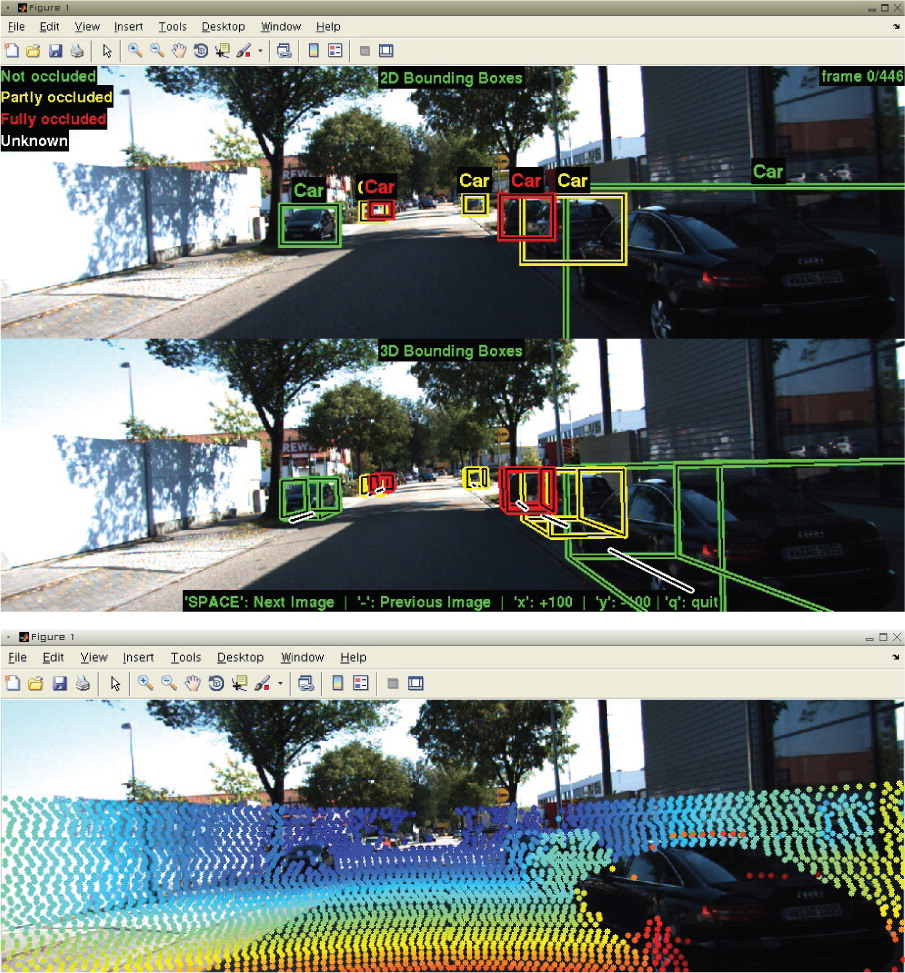
\includegraphics[width=0.45\textwidth]{images/kitti.jpeg}
%     \caption{Images with 2D and 3D bounding boxes and labels (top), Velodyne point clouds (bottom) and their projections onto the image plane.}
%     \label{fig:kitti}
% \end{figure}

\begin{wrapfigure}{L}{0.5\textwidth}
    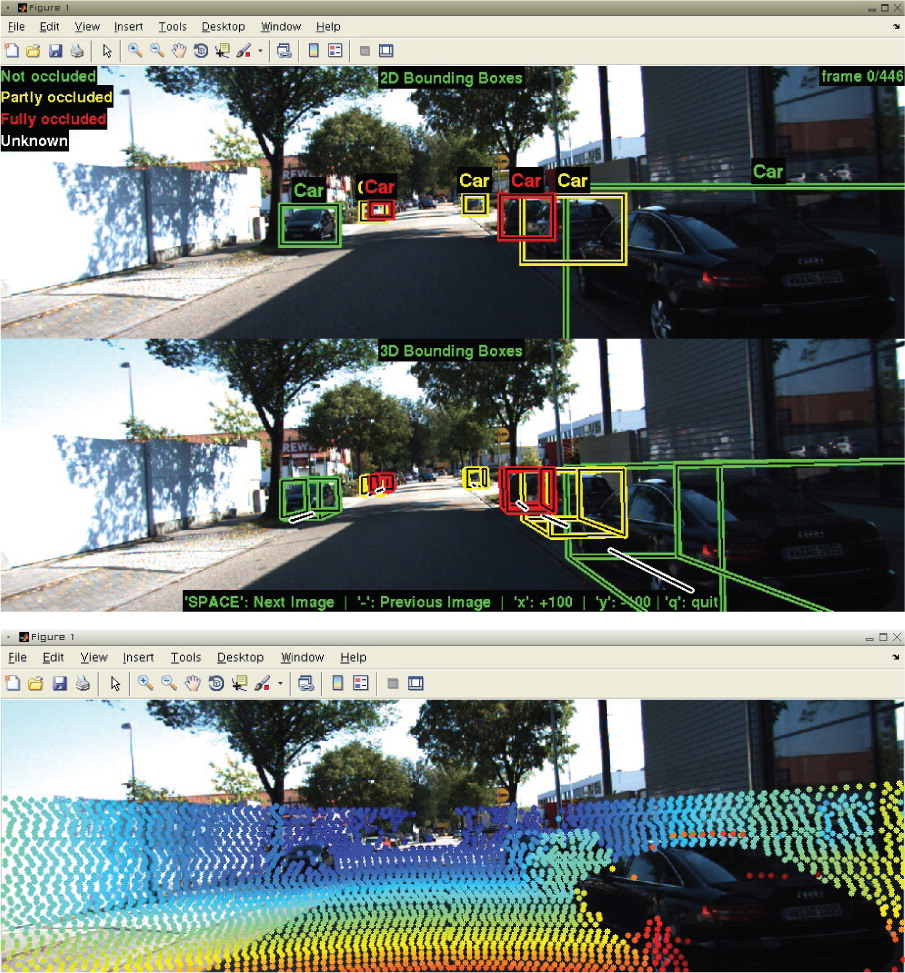
\includegraphics[width=0.47\textwidth]{images/kitti.jpeg} 
    \caption{Images with 2D and 3D bounding boxes and labels (top), Velodyne point clouds (bottom) and their projections onto the image plane~\cite{kitti}.}
    \label{fig:kitti}
\end{wrapfigure}

Real world datasets are acquired by using sensors such as LiDARs and RGB-D cameras. This implies the presence of noise because real-world sensors are imperfect, and acquiring data from the real world is a difficult task. Both indoor and outdoor dataset can be found.

An example of indoor dataset is S3DIS~\cite{s3dis}, a large-scale dataset composed of colored 3D scans, that are points with 3D coordinated and RGB color values, of indoor areas of large building with various architectural styles.

Outdoor datasets can vary on the type of scene acquired, but most datasets are taken in urban environments, since this type of data is particularly interesting in the context of autonomous driving.

% \begin{figure}[H]
%     \centering
%     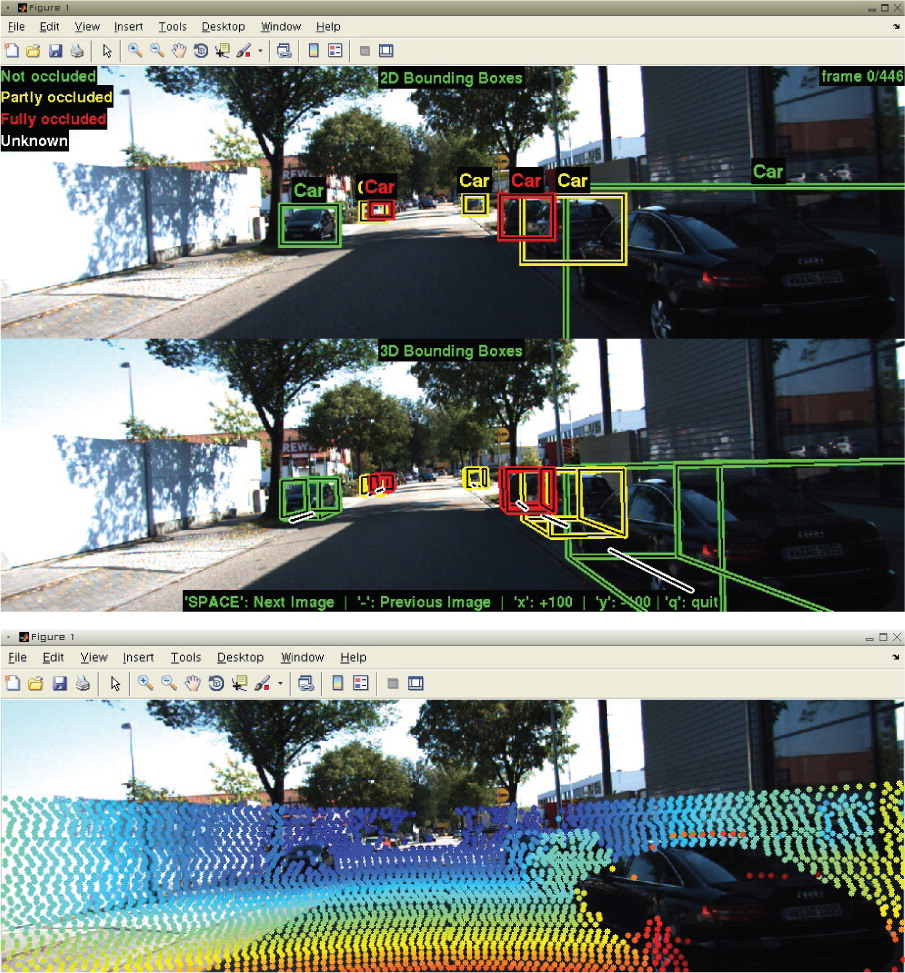
\includegraphics[width=0.4\textwidth]{images/kitti.jpeg}
%     \caption{Images with 2D and 3D bounding boxes and labels (top), Velodyne point clouds (bottom) and their projections onto the image plane.}
%     \label{fig:kitti}
% \end{figure}

The most notable example of outdoor dataset acquired with autonomous driving in mind is KITTI~\cite{kitti}: data is captured from a VW station wagon, an autonomous driving platform with two high-resolution color and grey cameras, a Velodyne laser scanner and a GPS localization system. Scenarios include real-world traffic on freeways in rural areas or inner-city scenes with many static and dynamic objects. For each sequence data include raw data, object annotations in form of 3D bounding box tracklets and a calibration file. For each dynamic object within the reference camera's field of view, the 3D bounding boxes classify objects in the classes 'Car', 'Van', 'Truck', 'Pedestrian', 'Person', 'Cyclist', 'Tram' and 'Misc'; each object has a class and its 3D size. For each frame it's available the object's translation and rotation in 3D in the Velodyne coordinates, along with the level of occlusion and truncation.
An example of a scene recorded from this dataset is shown in figure~\ref{fig:kitti}.


% \paragraph{S3DIS~\cite{s3dis}}

% S3DIS (Standford 3D Indoor Scene Dataset) is a large-scale dataset composed of colored 3D scans, that are points with 3D coordinated and RGB color values, of indoor areas of large building with various architectural styles. S3DIS contains 5 large-scale indoor scenes from three buildings. The point clouds are automatically generated without manual intervention.

% The buildings are parsed into spaces that are semantically meaningful with a hierarchical parsing method. To parse point clouds into disjoint spaces the void-based approach was followed: the void spaces are detected using a density histogram and this forms a signature of the point cloud. Then, it was chosen a unique $xyz$ reference frame for the buildings, normalized in a cube. The disjoint spaces are then parsed into elements with labels.

% \begin{figure}[ht]
%     \centering
%     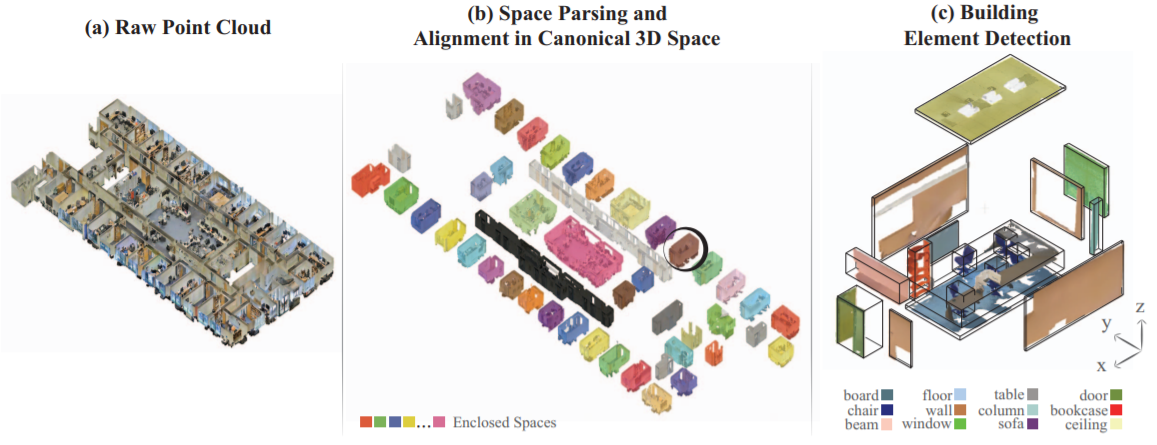
\includegraphics[width=0.8\textwidth]{images/s3dis.png}
%     \caption{S3DIS: Semantic parsing of a large-scale point cloud.}
%     \label{fig:s3dis}
% \end{figure}

% \paragraph{Semantic3D~\cite{hackel2017semantic3dnet}}

% Semantic3D is the largest 3D point cloud dataset with terrestrial laser scans and semantic ground truth annotation, scenes are for example farms, town halls, sport fields, castles and market squares. It has over 4 billions points  collected from around 110000 $m^2$ area with a static LiDAR, and class labels for 8 classes (man made terrain, natural terrain, high vegetation, low vegetation, buildings, remaining hard scale, scanning artifacts, cars and trucks).

% The class labels have been manually assigned to each point, this strategy permitted to not inherit errors from the segmentation approach. The manual labelling can be done in 3D, selecting few points and fitting a simple model to label the object, or in 2D, rotating the point cloud to fix a view and draw closed polygons to detect objects.

% \paragraph{ScanNet~\cite{dai2017scannet}}

% It is a dataset of richly-annotated RGB-D scans of real-world environments containing 2.5 millions RGB-D images in 1513 scans acquired in 707 distinct spaces; this dataset is annotated with estimated calibration parameters, camera poses, 3D surface reconstructions, textured meshes, dense object-level semantic segmentations, and aligned CAD models. ScanNet contains spaces such as offices, apartments, and bathrooms, ranging from small to large spaces.

% Data are collected as videos through handheld devices such as iPhone or iPad with an attached RGB-D sensor. The semantic annotation is done with Amazon Mechanical Turk for instance-level object category labeling and 3D CAD model alignment. The framework used to acquire data runs in an unsupervised way so it continues to grow.

% \paragraph{KITTI~\cite{kitti}}

% KITTI is among the most famous benchmarks with 3D data. Data are captured from a VW station wagon, an autonomous driving platform with two high-resolution color and grey cameras, a Velodyne laser scanner and a GPS localization system, for use in mobile robotics and autonomous driving research, data are used for 3D object detection, tracking and scene flow estimation. Scenarios include real-world traffic on freeways in rural areas or inner-city scenes with many static and dynamic objects.

% The dataset includes camera images, laser scans, high-precision GPS measurements and IMU accelerations (i.e. a specific type of sensor that measures angular rate, force and sometimes magnetic field) from a combined GPS/IMU system. The raw data are divided into the categories 'Road', 'City', 'Residential', 'Campus' and 'Person'; for each sequence data include raw data, object annotations in form of 3D bounding box tracklets and a calibration file. For each dynamic object within the reference camera's field of view, the 3D bounding boxes classify objects in the classes 'Car', 'Van', 'Truck', 'Pedestrian', 'Person', 'Cyclist', 'Tram' and 'Misc'; each object has a class and its 3D size. For each frame it's available the object's translation and rotation in 3D in the Velodyne coordinates, along with the level of occlusion and truncation.

% \paragraph{nuScenes~\cite{caesar2020nuscenes}}

% nuScense (nuTonomy scenes) carries the full autonomous vehicle sensor suite: 6 cameras, 5 radars and 1 LiDAR, all with full 360 degree field of view. The dataset includes 1000 scenes of 20 seconds, each fully annotated with 3D bounding boxes from 23 classes and 8 attributes, The scenes include high traffic density such as intersections and construction sites, rare classes such as ambulances and animals, potentially dangerous traffic situations, such as jaywalkers or incorrect behaviors, maneuvers such as lane change, turning and stopping, and difficult situations for computer vision. The scenes are annotated by expert annotators with textual descriptions. Every object in a keyframe sampled from the scenes is labelled by experts with one of the 23 classes, semantic categories, and attributes (visibility, acitivity and pose), and a cuboid with $xyz$ coordinates, width, length, height and yaw angle.

% \paragraph{WaymoOpen~\cite{sun2020scalability}}

% This dataset consists of 1150 scenes of 20 seconds each, consisting of 5 LiDAR sensors and 5 pinhole camera data captured in urban and suburban geographies; data are annotated with 2D and 3D bounding boxes. For every label in LiDAR and camera data the dimensions of bounding boxes are defined.

% \begin{figure}[ht]
%     \centering
%     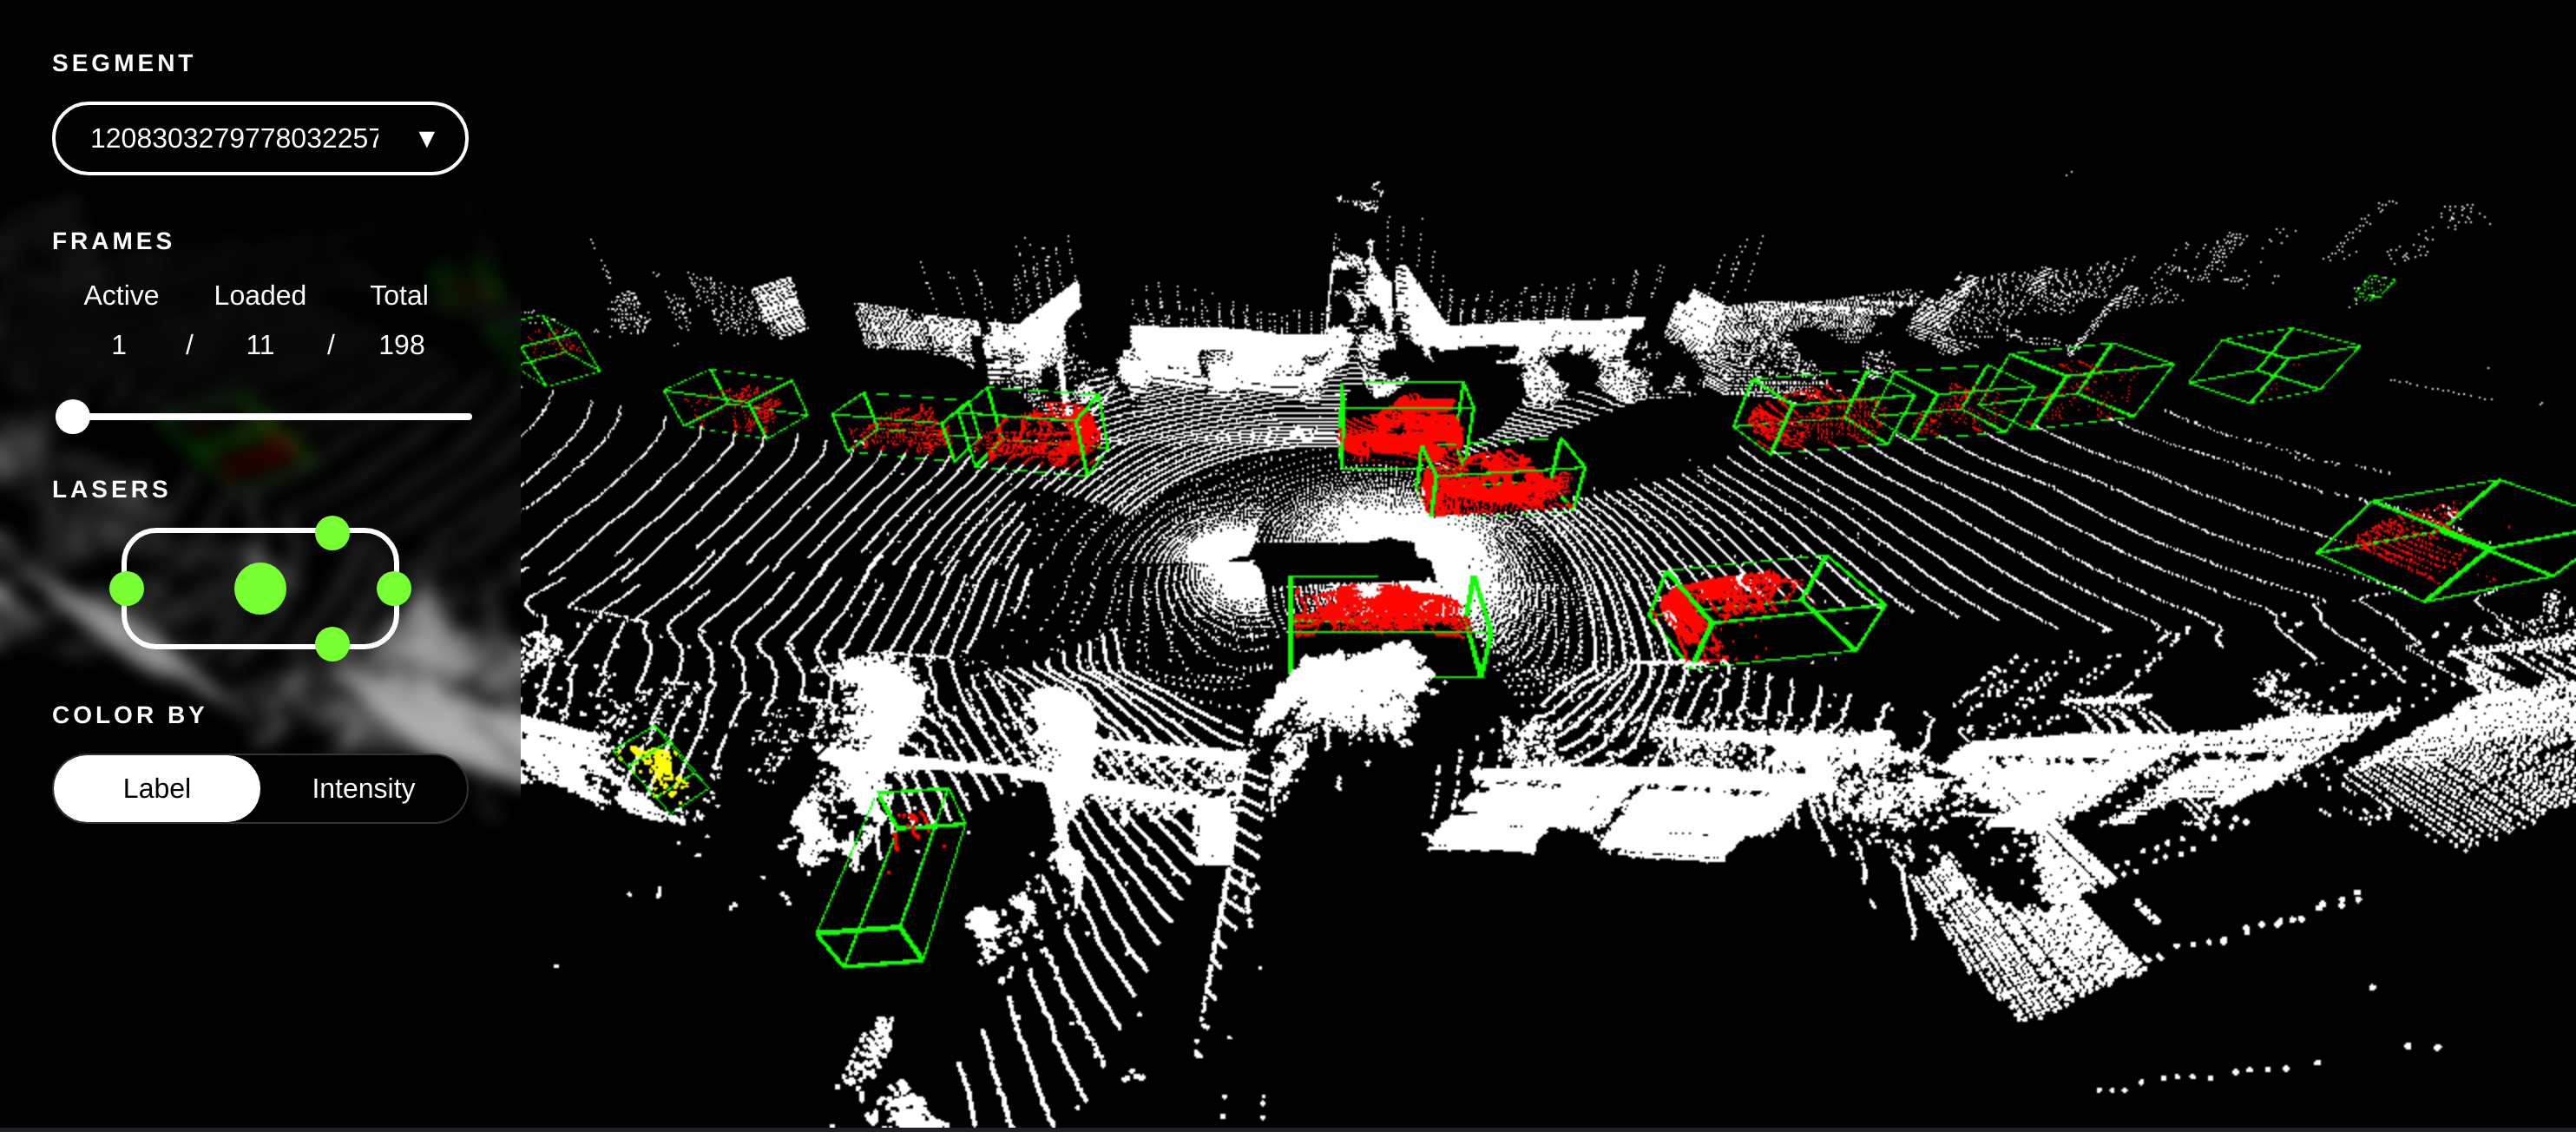
\includegraphics[width=0.8\textwidth]{images/waymo.png}
%     \caption{LiDAR label example in Waymo dataset.}
%     \label{fig:waymo}
% \end{figure}

% Vehicles, pedestrians, signs and cyclist in LiDAR data are exhaustively annotated: every object is labeld with $cx$, $cy$, $cz$, the center coordinated, $l$, $w$, $h$, the length, width and height, $\alpha$, the heading angle of the bounding box. Vehicles, pedestrians and cyclist are also annotated in camera data, with a bounding box defined by $cx$, $cy$, $l$, and $w$.

\subsection{Metrics}
\label{subsec:metrics}

Metrics are needed in order to compare performances of different algorithms; different evaluation metrics have been proposed for every tasks in point cloud understanding, so it is important to choose the appropriate ones (\cite{lu2020deep},~\cite{guo2020deep}).

For the task of \textbf{3D shape classification} the most commonly used metrics are the \textit{Overall Accuracy (O.A.)} and the \textit{Mean Class Accuracy (mACC)}. The O.A. is defined as the accuracy on the entire dataset and indicates how many predictions are correct over all predictions; the O.A. is defined in~\ref{eq:oa}.

\begin{equation}
\label{eq:oa}
    O.A. = \frac{TP+TN}{|dataset|}=\frac{TP+TN}{TP+TN+FP+FN}
\end{equation}

mACC is the mean of the accuracy of every class, defined in~\ref{eq:macc}.

\begin{equation}
\label{eq:macc}
    mACC = \frac{1}{C} \sum\limits_{c=1}^C Accuracy_c
\end{equation}

where $C$ is the number of classes in the dataset.

% The task of \textbf{3D point cloud segmentation} shares with the previous one two metrics, that are O.A. and mAcc, but it's common to use \textit{Mean Intersection Over Union (mIoU)}, too. Intersection Over Union, or IoU, used often on bounding boxes, is defined as the ratio between the area of overlap between two bboxes (intersection) and the area of union between the two bboxes. The mIoU is defined as the mean of IoU on all classes.

% Other used metrics, common also in other point cloud understanding tasks, are \textit{Precision} and \textit{Success} and their average counterpart. They are defined as:

% \[\begin{array}{c}
%      Precision = \frac{TP}{TP+FP}  \\
%      \\
%      Recall = \frac{TP}{TP+FN}
% \end{array}\]

% In other tasks such as 3D single and multi-object tracking two used metrics are \textit{AMOTA (Average Multi-Object Tracking Accuracy)}, \textit{AMOTP (Average Multi-Object Tracking Precision)}. In \textbf{Scene estimation} and \textbf{3D match and registration} commonly used metrics are \textit{End Point Error (EPE)} and \textit{ROC Curves}.

% In addition to these techniques, it is always suggested to visualize result as it is always an effective supplement of numbers.
  

\section{Classification Methods}

\subsection{Projection based}
Projection-based methods project the unstructured 3D point clouds into a specific presupposed modality (e.g. multi-view, voxels, pillars..), and extract features from the target format, which allows them to benefit from the previous research findings in the corresponding direction. In particular we analyze the multi-view representation approach, which can take advantage of the vast literature on computer vision, and the volumetric representation approach.

While intuitively it seems logical to build 3D shape classifiers directly from 3D models, in this section it is shown how an approach based on 2D images can actually dramatically outperform classifiers built directly on the 3D representations. In particular, a convolutional neural network trained on a fixed set of rendered views of a 3D shape and only provided with a single view at test time increases category recognition accuracy by a remarkable 8\% (77\% → 85\%) over the best models trained on 3D representations (in 2015). With more views provided at test time, its performance further increases. One of the main reasons for this performance increment is that by using a voxel-based representation the resolution needs to be significantly reduced in order to face the cubic spacial resolution. For example, 3D ShapeNets~\cite{ShapeNets} use a coarse representation of
shape, a 30×30×30 grid of binary voxels. In contrast, a single projection of the 3D model of the same input size corresponds to an image of 164×164 pixels, or slightly smaller if multiple projections are used. In addiction to this, must be taken into account that using 2D images allows to benefit from massive image databases, pre-existing CNN architectures which can be fine tuned and a wide literature on image descriptors.

\subsubsection{Multi-View}
%TODO in generale mettere la citazione quando si parla di qualcosa in tutta la sezione

As introduced before, the simple strategy of classifying views independently works remarkably well, but the focus of this section is to explain new ideas for how to “compile” the information in multiple 2D views of an object into a compact object descriptor using a new architecture called multi-view CNN. The multi-view CNN learns to combine the views instead of averaging, and thus can use the more informative views of the object for prediction while ignoring others. The multi-view approach, in the image classification context, is related to “jittering” (or data augmentation) as the different views can be seen as jittered copies. The method that will be described in fact can be also applied to jittered copies and can outperforms standard CNNs trained with the same jittered copies (for example on the sketch recognition benchmark~\cite{eitz2012hdhso}).

Let's start from the data: the view-based representations start from multiple views of a 3D shape, generated by a rendering engine. As said before, we could simply average the descriptors obtained from these views (that are all considered equally important) and obtain good results. Another approach is to concatenate all the different views and obtain a single big compact descriptor, but in this case we need to always respect the same point of views order and applying this order is not always possible, because the pose of the objects must be the expected one or correctly deduced.
The approach we'll describe, instead, learns to combine information from multiple views using a unified CNN architecture that includes a view-pooling layer.

\paragraph{Input}
In order to generate the different views of a 3D object, given its point cloud representation, we essentially need to preprocess the data with two steps: 
we connect the points and obtain edges forming faces (not necessary if the 3D models in the database is stored as polygon meshes) and in order to generate rendered views of
polygon meshes we need to use a reflection model (in the described approach is used the the Phong reflection model). Next we can apply the perspective projection and uniformly scale shapes to fit into the viewing volume. 
Two different cameras setup were experimented:\begin{itemize}
\item {\textbf{Camera setup 1: } is assumed that the input shapes are upright oriented, as the most online database are. 12 cameras, each every 30 degrees, elevated 30 degrees from the ground plane point toward the centroid of the mesh. See the left side of figure \ref{fig:multiview}.}
\item {\textbf{Camera setup 2: } the previous assumption about the upright orientation is eliminated so we need more views to ensure a good representation. 20 cameras pointing toward the centroid of the mesh are placed at the 20 vertices of an icosahedron enclosing the shape. Then, for each camera is taken a view using 0, 90, 180, 270 degrees rotation along the axis passing through the camera and the object centroid. This camera setup therefore has a total of 80 views.}
\end{itemize}

\begin{figure}[ht]
    \centering
    \captionsetup{width=.8\linewidth}
    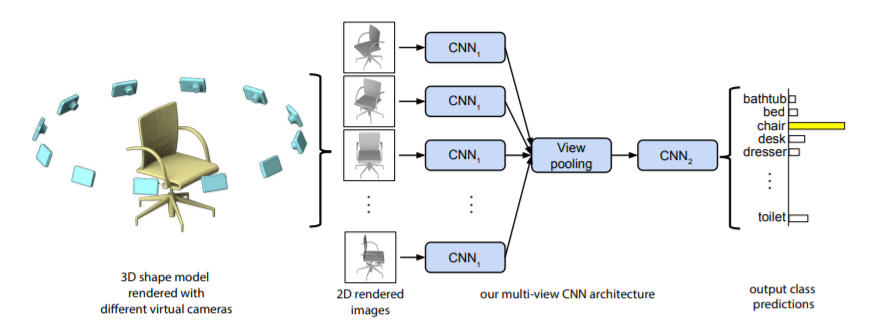
\includegraphics[width=0.8\textwidth]{images/multiview.png}
    \caption{ Multi-view CNN for 3D shape recognition (illustrated using the 1st camera setup). At test time a 3D shape is rendered from 12
different views and are passed thorough CNN1 to extract view based features. These are then pooled across views and passed through
CNN2 to obtain a compact shape descriptor.}
    \label{fig:multiview}
\end{figure}

\paragraph{Architecture}
\textbf A simple approach is to fine-tune a pre-trained CNN using the different views, obtaining a descriptor for each view. Then we train one-vs-rest linear SVMs (each view is treated as a separate training sample) to classify shapes using their image features. At test time, we simply sum up the SVM decision values over all 12 views and return the class with the highest sum. Alternative approaches like averaging image descriptors, lead to worse accuracy.

Let's describe now an approach that  \textbf{learns to aggregate views: MVCNN}. The input of the network are the different views of the 3D object. Each of these views is passed through the the first part of the network (CNN1) that is formed by 5 convolutional layers. Consequently the quantity of branches is equal to the quantity of views. The feature maps in output from this part are then aggregated at a viewpooling layer into a single feature map. At the end of the architecture (CNN2) we have 3 fully connected layers. See figure \ref{fig:mvcnn} to visualize the structure and table \ref{fig:MVCNN_TABLE} for layers details.

\begin{figure}[ht]
    \centering
    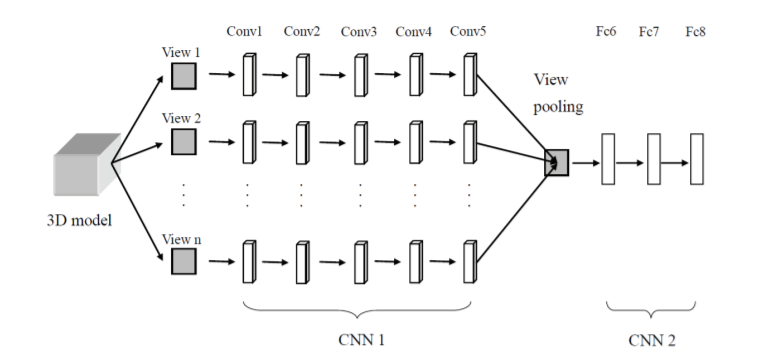
\includegraphics[width=0.8\textwidth]{images/mvcnn.png}
    \caption{Architecture of MVCNN model.}
    \label{fig:mvcnn}
\end{figure}

\begin{figure}[ht]
    \centering
    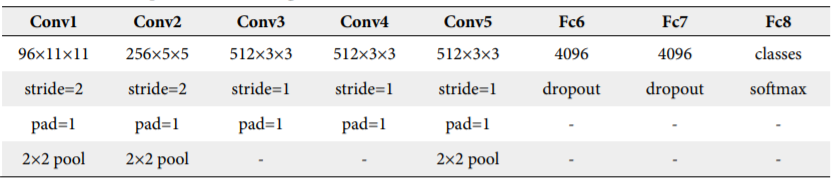
\includegraphics[width=0.8\textwidth]{images/MVCNN_TABLE.png}
    \caption{ Details on parameters of the MVCNN.}
    \label{fig:MVCNN_TABLE}
\end{figure}
\newpage

All branches in the first part of the network share the same parameters in CNN1. The view-pooling layer uses element-wise max pooling strategy to combine the discriminative information of multiple views and increase the computational efficiency. The viewpooling method is similar to traditional max-pooling operation. An alternative is element-wise mean
operation, but it is not as effective. The view-pooling layer can be placed anywhere in the network but experiments show that setting it after the 5th convolutional layer is the best choice. The MVCCN is fine-tuned for classification, but using a Mahalanobis metric W that directly projects the output descriptor $\phi \in \mathbb{R}^d$ to $W(\phi) \in \mathbb{R}^p$ and calculating the $l_2$ distance in the projected space we obtain a significant boost to retrieval performance.

An MVCNN can also be used as a simple 2D image classifier instead of CNN. If we use data augmentation and feed the MVCNN with all the different jittered copies and the original image we can obtain better results than using a CNN (experiments are reported in ~\cite{multi_view} on the sketch recognition benchmark~\cite{eitz2012hdhso}).

\paragraph{Results}
The dataset used is ModelNet40, described in section \ref{ModNet40}. The table in figure \ref{fig:MVCNN_results_table} compares different settings of MVCNNs to other approaches like SPH(Spherical Harmonics descriptor), LFD (LightField descriptor) and 3D ShapeNets on the ModelNet40 dataset. See also the retrieval precision-recall curves in figure \ref{fig:MVCNN_prec_rec_curve}.

\begin{figure}[ht]
    \centering
    \captionsetup{width=.8\linewidth}
    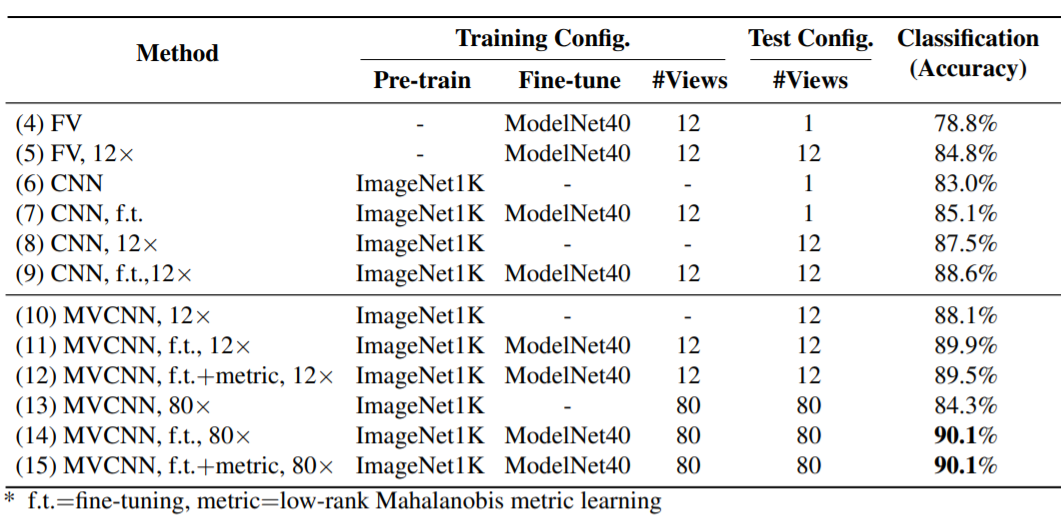
\includegraphics[width=0.8\textwidth]{images/MVCNN_results_table.png}
    \caption{ Classification and retrieval results. FV is another simpler approach described in the same paper that describes MVCNNs based on Fisher Vectors.}
    \label{fig:MVCNN_results_table}
\end{figure}

\begin{figure}[ht]
    \centering
    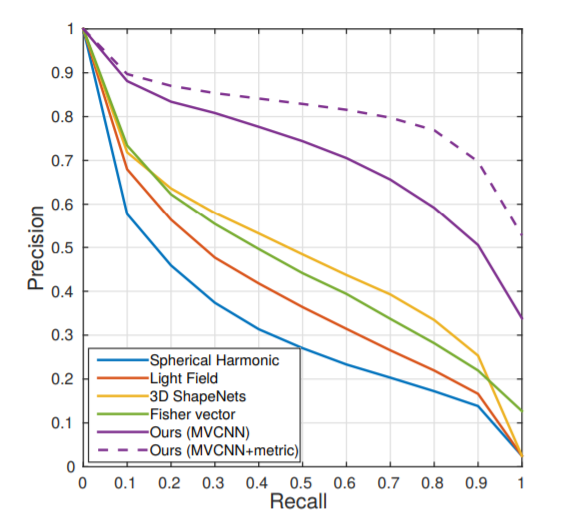
\includegraphics[width=0.5\textwidth]{images/MVCNN_prec_rec_curve.png}
    \caption{ Retrieval precision-recall curves.}
    \label{fig:MVCNN_prec_rec_curve}
\end{figure}

\paragraph{Saliency map among views}
Since this approach learns to aggregate views in a single network it is possible to trace back to the influence of the different views on the MVCNN output score $F_c$ for its ground truth class $c$. For each 3D shape $S$ and its relative views $\{I_1, I_2, ... I_K\}$ we can compute $w$ of the following equation using backpropagation

\begin{equation}
    [w_1, w_2, ... w_K] = \bigg[
    \frac{\partial F_c}{\partial I_1}\Bigr|_{\substack{S}},
    \frac{\partial F_c}{\partial I_2}\Bigr|_{\substack{S}},
    ... 
    \frac{\partial F_c}{\partial I_K}\Bigr|_{\substack{S}}
    \bigg]
\end{equation}

and obtain saliency maps for individual views. Some examples are reported in figure \ref{fig:MVCNN_saliency}.

\begin{figure}[ht]
    \centering
    \captionsetup{width=.9\linewidth}
    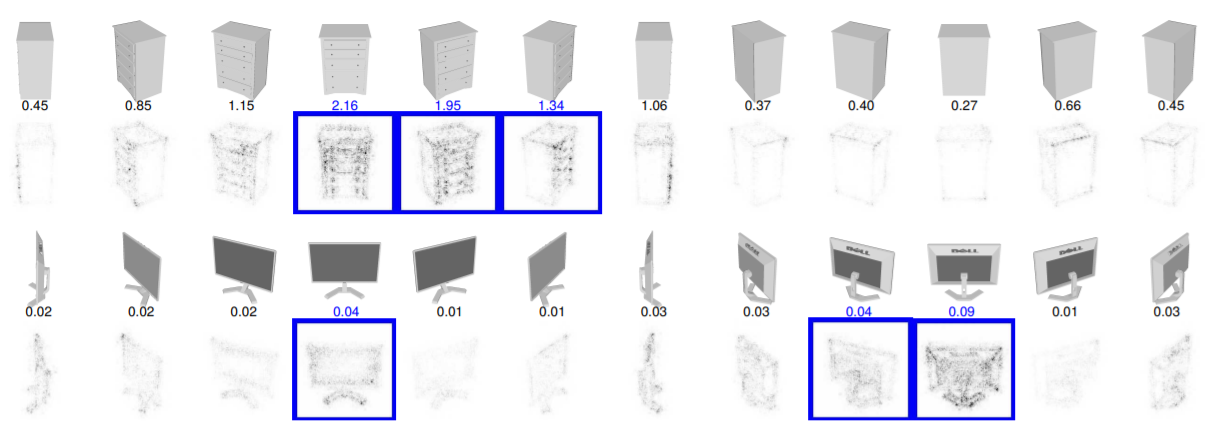
\includegraphics[width=0.9\textwidth]{images/MVCNN_saliency.png}
    \caption{Top three views with the highest saliency are highlighted in blue and the relative magnitudes of gradient energy for each view is
shown on top. The saliency maps are computed by back-propagating the gradients of the class score onto the image via the view-pooling
layer. Notice that the handles of the dresser and of the desk are the most discriminative features. (Figures are enhanced for visibility.)}
    \label{fig:MVCNN_saliency}
\end{figure}



% possibili approfondimenti:
%- Phong reflection model (https://users.cs.northwestern.edu/~ago820/cs395/Papers/Phong_1975.pdf)
%- Learning-based Multiple Pooling Fusion (https://s3.ap-northeast-2.amazonaws.com/journal-home/journal/jips/fullText/302/13.pdf)
% Saliency map (https://arxiv.org/pdf/1312.6034.pdf)
 





\subsubsection{Volumetric} 
Since a point cloud is a 3D structure, it is quite natural using a 3D model as a projection space. In this section we will present an approach that projects the cloud points into a volumetric occupancy grids and, given these grids, performs the classification task using a 3D convolutional neural network: VoxNet.

\paragraph{Input}
The initial input of the algorithm is a point cloud segment, usually given by the intersection of a point cloud with a bounding box and may include background clutter. 

Each point $(x,y,z)$ of the point cloud is mapped to discrete voxel coordinates $(i,j,k)$. 
This mapping is obviously depending on the orientation, origin and resolution of the voxel grid in space. For the orientation it is assumed that the $z$ axis is aligned with the gravity direction, while the origin is supposed to be given as an input. How to deal with the remaining degree of freedom, the rotation around the $z$ axis? First method: it is possible to define a canonical orientation for each object and detect this orientation automatically, but this approach is often non-trivial in practise. Second method: using data augmentation at training time; in practise what we have to do is to create $n$ copies of each input instance, each rotated $360$\textdegree$/n$ around the $z$ axis. At testing time we pool the activations of the output layer over all $n$ copies. As mentioned, also grid resolution has influence on results: in the experiments a fixed occupancy grid $32 \times 32 \times 32$ voxels was used. We have to keep these dimensions small because the computational space increases cubically. To keep larger spatial extents in memory are used hierarchical data structures and copy specific segments to dense arrays as needed. 

There are three possible ways to model occupancy grids:
\begin{itemize}
\item \emph{Binary occupancy grid. } Each voxel has just two options, it can be occupied or unoccupied. Since data coming from sensors always is noisy a probabilistic approach is used to determine the voxel's binary state.
\item \emph{Density grid. } Identical to the previous one, except for the fact that each voxel is assumed to have a continuous, and not binary, density.
\item \emph{Hit grid. } Differently from the two previous approaches, this model only consider hits, and ignore the difference between unknown and free space. Hence the probabilistic approach is different.
\end{itemize}

\begin{figure}[ht]
    \centering
    \captionsetup{width=.9\linewidth}
    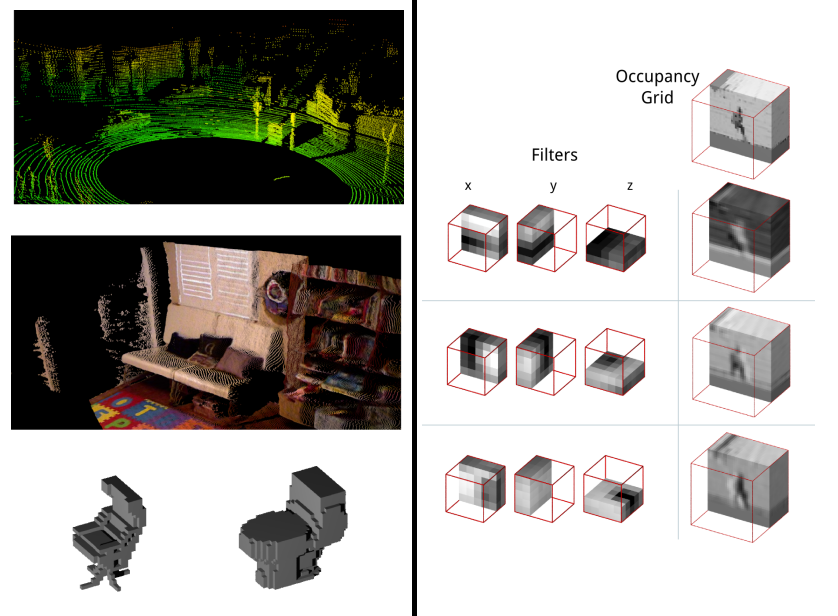
\includegraphics[width=0.72\textwidth]{images/VOLUM_cloud_filtpng.png}
    \caption{Left: From top to bottom, a point cloud from the Sydney Objects Dataset,
a point cloud from NYUv2, and two voxelized models from ModelNet40.
Right: Cross sections of three 5 × 5 × 5 filters from the first layer of VoxNet in the Sydney Objects Database, with corresponding feature map on the right.}
    \label{fig:VOLUM_cloud_filtpng}
\end{figure}

\paragraph{Architecture}
The input layer accepts a grid of $I \times J \times K$ voxels, as described before. In the performed experiments $I = J = K = 32$. Voxel entries are supposed to be normalized in the range $(-1,1)$.

After the input layer we have convolutional layers. The notation that will be used to describe these layers is $C(f,d,s)$, where $f$ is the number of filters, $d$ is the spatial dimension and $s$ is the stride. The output is passed through a leaky ReLU ($a(x)=max(0.1*x , x)
)$ with parameter 0.1.

Next we have pooling layers $P(m)$, used to downsample the input volume. We divided our input in blocks of $m \times m \times m$ and then take their maximum (we have a max-pooling operation).

At the end we have fully connected layers $FC(n)$, where $n$ is the number of output neurons. The activation function used are ReLUs and in the final layer it's used a softmax activation function.

An optimization of the hyperparameters leads to obtain the following network scheme:
$C(32, 5, 2) - C(32, 3, 1)-P(2)-F C(128)-F C(K)$, where $K$ is the number of classes (see figure \ref{fig:VoxNet_archtecture}). In total the model has $921736$ parameters, much less than a typical CNN for image classification. The authors of the paper think this is because point cloud classification is a simpler task, as many factors that images classifiers have to take into account (perspective, illumination, ...) are not present. Training details: SGD with momentum, L2 regularization, dropout, momentum parameter 0.9, initial LR=0.01 or 0.001 depending on the dataset.


It is also possible to use a multiresolution approach. In this case we use $r$ networks as described before, each of them corresponding to a resolution input grid. Then, at the fully connected layers, we merge informations coming from the different networks and obtain a single descriptor.

\begin{figure}[ht]
    \centering
    \captionsetup{width=.7\linewidth}
    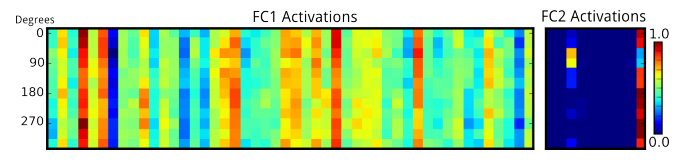
\includegraphics[width=0.6\textwidth]{images/VOLUM_invariance.png}
    \caption{Neuron activations for the two fully connected layers of VoxNet
when using the point cloud from figure \ref{fig:VoxNet_archtecture} (right) as input in 12 different
orientations.}
    \label{fig:VOLUM_invariance}
\end{figure}

\begin{figure}[ht]
    \centering
    \captionsetup{width=.9\linewidth}
    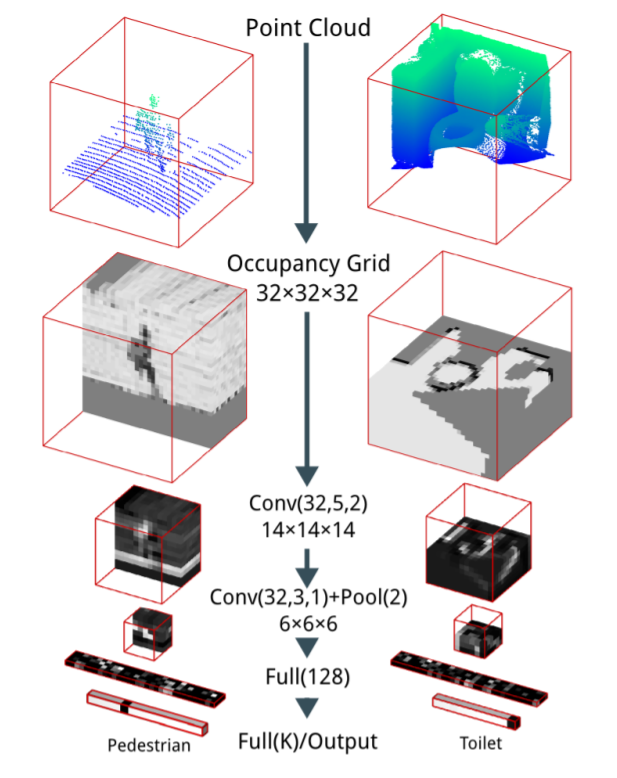
\includegraphics[width=0.4\textwidth]{images/VoxNet_archtecture.png}
    \caption{The VoxNet Architecture. We show inputs, example
feature maps, and predicted outputs for two instances from our experiments.
The point cloud on the left is from LiDAR and is part of the Sydney Urban
Objects dataset \cite{dataset_ICRA2012}. The point cloud on the right is from RGBD and is part of NYUv2 \cite{dataset_ECCV2012}.}
    \label{fig:VoxNet_archtecture}
\end{figure}

\paragraph{Results}
VoxNet was evalueted in three different domains: LiDAR point cloud, RGBD point clouds and CAD models as figure \ref{fig:VOLUM_cloud_filtpng} shows. In figure \ref{fig:VOLUM_results_table} are reported some results on different datasets and comparison to other approaches. 

\begin{figure}[ht]
    \centering
    \captionsetup{width=.9\linewidth}
    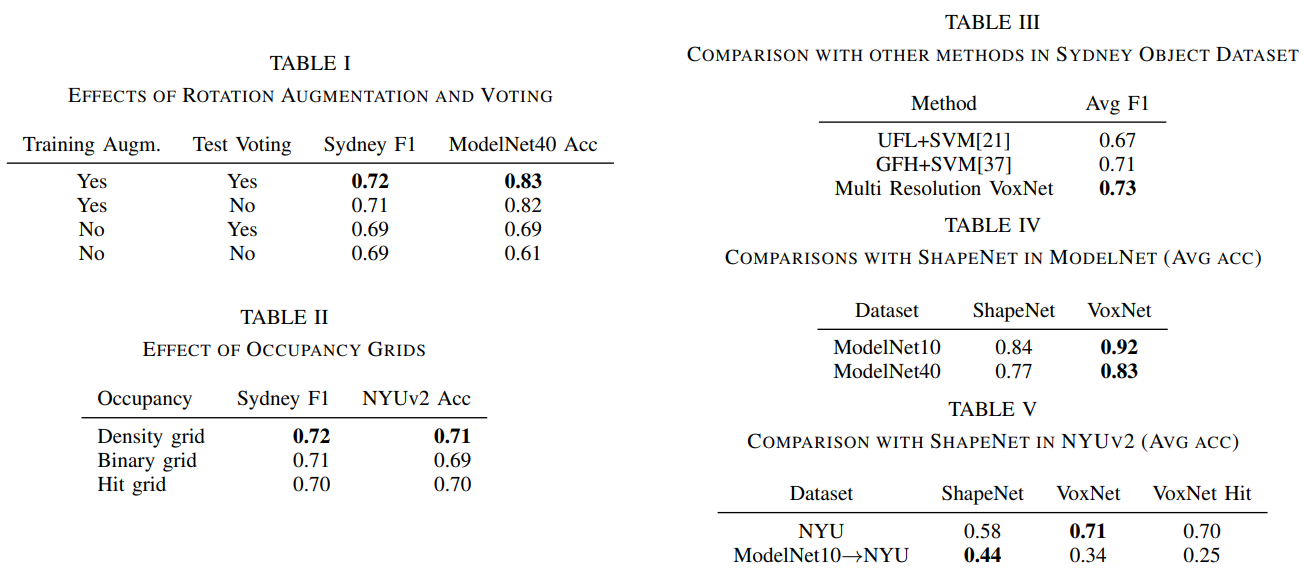
\includegraphics[width=0.9\textwidth]{images/VOLUM_results_table.png}
    \caption{Performance results on different datasets, and comparison to other approaches: UFL+SVM combines unsupervised Deep Learning with SVM; GFH+SVM designs a rotationally invariant descriptor and classifies it with a nonlinear SVM.}
    \label{fig:VOLUM_results_table}
\end{figure}

A qualitative result we can test is the rotational invariance. As explained before, the network was trained using data augmentation (pre-established rotation around $z$ axis). In order to verify if there is an effective rotational invariance we can analyze the activation of the two fully connected layers, given as input the same point cloud in different orientations. As we can see in figure \ref{fig:VOLUM_invariance}, 12 different rotation are analyzed and the corresponding neuron activation are very similar. This show that there is an approximate rotational invariance.

\subsection{Point Based}
Point-based methods learn features directly from the points and not from their spatial arrangement, as in projection based methods. These methods differ in the architecture and on the basis of that they can be divided in pointwise MLP, convolution-based, graph-based and hierarchical data structure-based. In this survey we will present MLP, convolution-based and graph-based methods.

\subsubsection{Multi-Layer Perceptron}

In pointwise MLP methods, features from every point of a point cloud are extracted with independent Multi-Layer Perceptrons and then aggregated with a symmetric function, such as max pooling, in a unique vector that represents the whole point cloud; the process is illustrated in figure~\ref{fig:mlp} (\cite{guo2020deep}). 

\begin{figure}[ht]
    \centering
    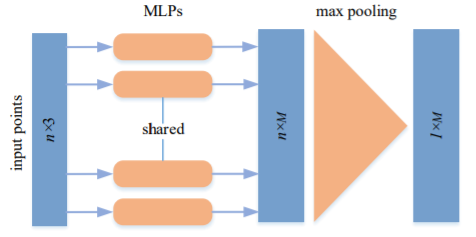
\includegraphics[width=0.5\textwidth]{images/mlp.png}
    \caption{Architecture of PointNet~\cite{guo2020deep}.}
    \label{fig:mlp}
\end{figure}

\paragraph{PointNet}
\label{par:pointnet}

A famous architecture that uses MLP and directly consumes point clouds, without transforming them in other structures, is PointNet~\cite{qi2017pointnet}, one of the early attempts to design a deep network for consumption of unordered 3D point sets; this model is used for the task of classification as well as segmentation, in fact PointNet takes as input point clouds and outputs their class labels for the entire cloud (classification) or per point (segmentation). The transformations of data made by projection-based models render the data unnecessarily voluminous while introducing quantization artifacts, point clouds directly used, instead, are easier to learn from because of their simple and unified structures. Points in a point cloud have not an intrinsic order, but the class that they represent must be invariant to permutations, so they need at least a symmetrization to be fed into the networks. 

A point cloud is a set of 3D points where each point is a three-dimensional vector, and can have other features such as color channels, that we don't consider. For the classification task the input point cloud is sampled from a shape or segmented from a scene, in this case the network outputs a score for each of the $k$ classes considered. For segmentation the input is a single object for region segmentation or a sub-volume of a scene, for this task the network outputs a score for each point and for each class.

A subset of points in an Euclidean space has three main properties: it is \textbf{unordered}, so the network that consumes $n$ points has to be invariant to $n!$ permutations of them; the points \textbf{interact} because they are immersed in a metric space and it has to be considered the distance between them and their neighborhood; the subset is \textbf{invariant under transformations} because rotating and translating points all together does not change the class the object belongs to.

\begin{figure}[ht]
    \centering
    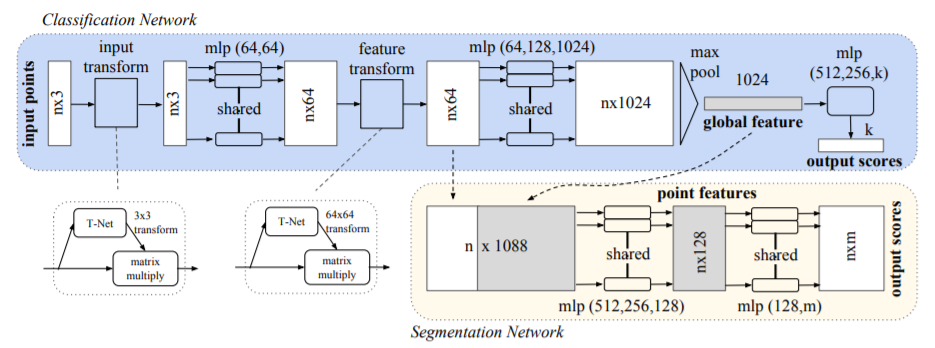
\includegraphics[width=\textwidth]{images/pointnet_architecture.png}
    \caption{Architectures of PointNet for classification and segmentation tasks~\cite{qi2017pointnet}.}
    \label{fig:pointnet_architecture}
\end{figure}

\paragraph{PointNet Architecture}

The input of the classification network of PointNet is a set of $n$ points, the network then applies a transformation of this set in many layers, as can be seen in figure~\ref{fig:pointnet_architecture}, and then aggregates features with max pooling; the global feature tensor is then passed through another MLP that produces $k$ scores, one for every class.

\paragraph{Joint Alignment Network}

To achieve invariance to rigid geometric transformations, under which the predicted label for the point cloud must be preserved, a simple solution is to align all input set to a canonical space; instead in PointNet the T-net showed in figure~\ref{fig:pointnet_architecture} is used: this mini-network is composed by point independent feature extractions, max pooling and fully connected layers. The T-net predicts an affine transformation matrix and applies it to the input points; another transformation matrix is applied later in the network, to the features space that has many more dimensions than the input space. The affine transformation matrices predicted by the T-net perform a \textit{pose normalization} to the point cloud, this also reduces the extent to which data augmentation is needed, because in point clouds the objects can take an infinite number of different poses. In order to improve optimization in such a big space, the matrix is constrained to be orthogonal by a regularization term added to the softmax training loss.

\paragraph{Symmetric Function for Unordered Input}

As previously said, the model has to be invariant to all points permutation, to achieve this objective PointNet uses a symmetric function that takes $n$ points and produces a new order-invariant vector. The idea on which is based the symmetric module of PointNet is that a generic function defined on an unordered set of points can be approximated by a function applied on the transformed points, shown in~\ref{eq:pointnet_symmetric}.

\begin{equation}
\label{eq:pointnet_symmetric}
    f(\{x_1, \dots ,x_n\}) \approx g(h(x_1), \dots , h(x_n))
\end{equation}

where $f : 2^{\mathbb{R}^N} \to \mathbb{R}$, $h: \mathbb{R}^N \to \mathbb{R}^K$ and $g: \overbrace{\mathbb{R}^K \times \dots \times \mathbb{R}^K}^{n \text{ times}} \to \mathbb{R}$ is a symmetric function. In the network $h$ is a multi-layer perceptron and $g$ a composition of a single variable function and a max pooling function. Using a collection of $h$ the approximated $f$, $[f_1, \dots, f_K]$, is produced and represents a global signature of the point set, invariant to points order. This method has a universal approximation ability proved with a theorem in~\cite{qi2017pointnet}, that means that PointNet as a neural network is capable of approximate continuous set functions (as it is $f$); in the worst case, with this method the network will produce a volumetric representation of point clouds by partitioning the space in equal-size voxel, but in practice it learns a better strategy.

\paragraph{Theoretical Analysis}

In~\cite{qi2017pointnet} the robustness of the network with respect to small perturbation of noise in points is proved: thanks to the architecture of the network and the chosen functions $h$ and $g$ defined above, for every set of points $S$ there exist two subsets $\mathcal{C}_S, \mathcal{N}_S \subseteq S$, such that for every set $T$, with $\mathcal{C}_S \subseteq T \subseteq \mathcal{N}_S$, it is true that $f(S) = f(T)$ and $|\mathcal{C}_S| \le K$, where $K$ is the dimension of the extracted features. In practice, $\mathcal{C}_S$ totally determines the output $f(S)$, for this reason it's called the \textit{critical point set} and its cardinality the \textit{bottleneck dimension of} $f$. This result shows that the extracted features from the point cloud remain unchanged if all the points of the critical point set are preserved and also with extra noise, up to $\mathcal{N}_S$, so PointNet is robust with respect to perturbation, corruption and extra noise points. In figure~\ref{fig:critical_point_sets} critical point sets and upper-bound shapes for many objects are visualized.

\begin{figure}[ht]
    \centering
    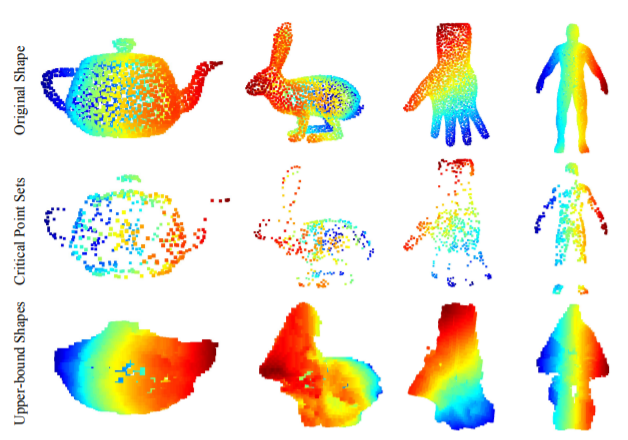
\includegraphics[width=0.6\textwidth]{images/critical_point_sets.png}
    \caption{Critical point sets and upper-bound shapes for unseen objects~\cite{qi2017pointnet}.}
    \label{fig:critical_point_sets}
\end{figure}

For the task of classification, the extracted global features are then passed through a simple MLP for output scores. For the task of segmentation, instead, the features pass through a new part of the network that's beyond the scope of this survey.

\paragraph{Results}

Validation experiments on PointNet has been made with dataset ModelNet40, described in this survey in~\ref{subsec:datasets}; PointNet has been the first MLP network tested on ModelNet40. From the mesh faces 1024 points are sampled uniformly and normalized in a unit sphere, then, during, training, these data are augmented with rotation and addition of Gaussian noise. The achieved mACC (section~\ref{subsec:metrics}) is $86.2 \%$, while the O.A. is $89.2 \%$.

These results are achieved with the whole PointNet network, but other experiments have been conducted to demonstrate the effectiveness of input and features transformations (T-net). The performance difference with or without T-net are summarized in figure~\ref{tab:t_net_accuracies}.

\begin{table}[ht]
    \centering
    \caption{Effects of input feature transformations on PointNet performances.}
    \begin{tabular}{cc|l}
        \hline \text { \textbf{Transform} } & \text { \textbf{Accuracy} (\%) } & \text {\textbf{Description} }\\
        \hline none & 87.1 & no T-net applied \\
        \hline input (3x3) & 87.9 & T-net applied only to input points (3x1)\\
        feature (64x64)  & 86.9 & T-net applied only to features (64x1)\\
        feature (64x64) + reg. & 87.4 & T-net applied only to feature points and regularization on training loss\\
        \hline
        both & 89.2 & T-net applied to input points and features \\
        \hline
    \end{tabular}
    \label{tab:t_net_accuracies}
\end{table}

To demonstrate robustness, the network has been tested in various types of input corruption scenarios: with $50 \%$ of missing points from the input, the accuracy drops by $2.4 \%$. At last, the analysis of space and time: PointNet has 3.5 millions parameters and has a computational cost of 440 millions FLOPs/sample (floating-point operations/sample); its space and time complexity is linear in the number of input points so it is very scalable.

\paragraph{PointNet++}
\label{par:pointnet++}

PointNet is limited because it cannot capture local structures and fine geometric structures from the neighborhood of each point, so Qi et al.~\cite{qi2017pointnet++} proposed a hierarchical network PointNet++, inspired by the fact that CNNs take features at different scales by a stack of convolutional layers.

PointNet learns a spatial encoding of each point and aggregates the points features in a global point cloud signature, but doing this it can't capture local structures induced by the metric of the space in which the point cloud is immersed. Using a hierarchical structure, as in CNNs, permits to progressively capture features at increasingly larger scales along a hierarchy and helps abstract local patterns to allow better generalization. PointNet++ has a \textit{local feature learner}, that is PointNet, that abstracts sets of points or local features, the weights of these local features are shared across the partitions of the point cloud, as in the convolutional setting. The partitions are overlapping local regions, defined as a neighborhood ball in the underlying Euclidean space.

\begin{figure}[ht]
    \centering
    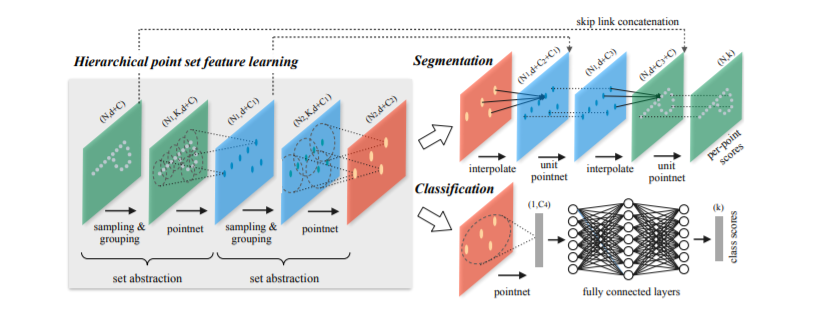
\includegraphics[width=\textwidth]{images/pointnet++_architecture.png}
    \caption{Architectures of PointNet++ for classification and segmentation tasks~\cite{qi2017pointnet++}.}
    \label{fig:pointnet++_architecture}
\end{figure}

\paragraph{Hierarchical Point Set Feature Learning}

As it is shown in figure~\ref{fig:pointnet++_architecture}, PointNet++'s structure is composed by set abstraction levels, in which the set of points is abstracted and a new smaller set is produced. Every set abstraction is composed of a \textit{Sampling}, a \textit{Grouping} and a \textit{PointNet} layer.

The Sampling layer selects a set of points from the input that will be the set of centroids of local regions; \textit{iterative farthest point sampling} (FPS) is used to choose the subset of centroids from the input set: a point is chosen to be a centroid if it's the most distant point, with respect to the metric, from the centroids previously chosen than the other points in the set. The Grouping layer builds local regions by computing the neighborhood of the centroids; the neighborhood of a centroid is built with all the points that are within a radius with respect to the metric distance (while in CNN the distance between pixels is defined by Manhattan's distance). Another way to construct centroids neighborhoods is k-NN search, but the first method guarantees a fixed region scale, making local region feature more generalizable across space. The \textit{PointNet layer} extracts feature vectors from the local regions; the input sets are the outputs of the Grouping layer, so they have different dimensions for every abstraction set, but PointNet is capable of extract fixed-length feature vectors from sets of different dimensions. Each local region is abstracted by a centroid and local feature that encodes the centroid's neighborhood, and the coordinates of points of a local region are first translated in a local frame relative to the centroid, in this way the network captures point-to-point relations in local regions.

\begin{figure}[ht]
    \centering
    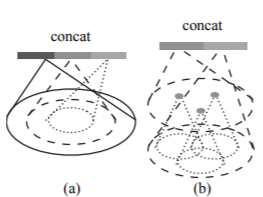
\includegraphics[width=0.4\textwidth]{images/density_adaptive_pointnet.png}
    \caption{(a) Multi-scale grouping (MSG); (b) Multi-resolution grouping (MRG)~\cite{qi2017pointnet++}.}
    \label{fig:density_adaptive_pointnet}
\end{figure}

\paragraph{Robust Feature Learning under Non-Uniform Sampling Density}

The problem of non-uniform sampling density is faced in~\cite{qi2017pointnet++}, in fact features learned in dense data may not be generalized in the case of sparse data available. In the case of low density areas it is not possible to inspect closely the point cloud, so larger scale patterns are looked for. To solve this problem, some \textit{density adaptive PointNet layers} are added to PointNet++ architecture, these layers learn to combine features from different scale regions when the density is different. So, instead of having a single scale for each abstraction level, as said above, in PointNet++ an abstraction level extracts multiple scales of local patterns and combines them intelligently according to local point density, this happens thanks to the density adaptive PointNet layers. 

There are two types of density adaptive layers, shown in figure~\ref{fig:density_adaptive_pointnet}: \textit{Multi-scale grouping} and \textit{Multi-resolution grouping}. MSG layers apply grouping layers with different scales followed by an application of PointNet to extract features at each scale, then features at different scales are concatenated to form a multi-scale feature vector; MSG approach is computationally expensive since it runs local PointNets at large scale neighborhoods for every centroid. MRG layers at every level $L_i$ build a concatenation of two vectors, the first one summarizes the features at every subregion from the previous features level in the network $L_{i-1}$ using the set abstraction level, the second one is obtained by processing all raw points in the local region at level $L_i$ with PointNet; when the density of a local region is low, the first vector is less reliable, but the second one is weighted higher, furthermore, when the density is high, the first vector have information of finer details.

\paragraph{Results}

PointNet++ has been evaluated on different datasets (2D objetcs, 3D objects, rigid and non-rigid objects,  real 3D scenes), including ModelNet40. All the point sets are normalized to be zero mean and within a unit ball, the architecture evaluated consists in a three-level hierarchical network with three fully connected layers. The overall accuracy achieved on ModelNet40 shape classification is $91,9 \%$.

\begin{figure}[ht]
    \centering
    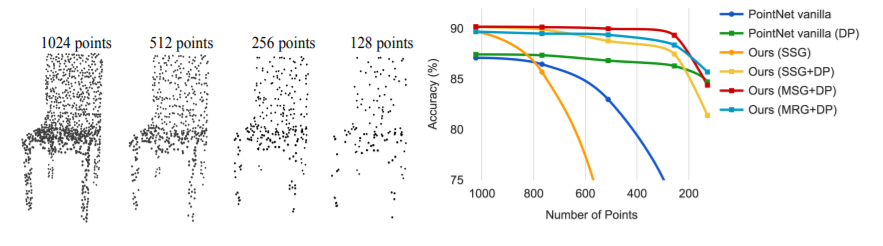
\includegraphics[width=0.9\textwidth]{images/pointnet++_density_robustness.png}
    \caption{Left: point cloud with random point dropout. Right: accuracy w.r.t. non-uniform density~\cite{qi2017pointnet++}.}
    \label{fig:pointnet++_density_robustness}
\end{figure}

PointNet++ is more robust to density variations, in fact some points are randomly dropped during training to learn an optimized strategy to combine the multi-scale features. In figure~\ref{fig:pointnet++_density_robustness} it is shown the robustness of PointNet++ with MSG or MRG, and DP (random dropout), with respect to PointNet.

\subsubsection{Convolutional Neural Networks}
The convolution operator is defined on two functions $f(\mathbf{x})$ and $g(\mathbf{x})$, with $\mathbf{x} \in \mathbb{R}^{d}$: 

\begin{equation}
    (f * g)(\mathbf{x})=\iint_{\boldsymbol{\tau} \in \mathbb{R}^{d}} f(\boldsymbol{\tau}) g(\mathbf{x}+\boldsymbol{\tau}) d \boldsymbol{\tau}
\end{equation}

In images the function $g(\mathbf{x})$ is a 2D function, and because images are made up by a discrete and fixed grid of pixel the integrals can be seen as the discrete sum of product between $f$ and $g$.

Such a regular structure is not intrinsic of point clouds, and thus convolution is not as easily implemented.

To tackle this problem without using an intermediate representation of the point cloud (as seen with projection based approaches) specialized convolution operators have been proposed.

In this section the PointConv operation, proposed by Wenxuan Wu et al~\cite{PointConv}, will be explored.

\paragraph{PointConv}

A point cloud is a set of 3D points $(x,y,z)$, so the 3D convolution can be written as: 

\begin{equation}
    \begin{array}{l}
\operatorname{Conv}(W, F)_{x y z}= 
\quad \iiint_{\left(\delta_{x}, \delta_{y}, \delta_{z}\right) \in G} W\left(\delta_{x}, \delta_{y}, \delta_{z}\right) F\left(x+\delta_{x}, y+\delta_{y}, z+\delta_{z}\right) d \delta_{x} d \delta_{y} d \delta_{z}
\end{array}
\end{equation}

where $W(\delta_{x}, \delta_{y}, \delta_{z})$ is the weight function and $F\left(x+\delta_{x}, y+\delta_{y}, z+\delta_{z}\right)$ is the feature of a point in the local region $G$ centered in  $p = (x,y,z)$.

Point clouds, unlike images, are not uniformly sampled from the 3D space: the points $(\delta_{x}, \delta_{y}, \delta_{z})$ do not have a fixed structure in the local region, so there could be subregions with more dense sampling and subregions with more sparse points, thus transforming the integral into a discrete sum is not trivial.
To deal with the uneven sampling the authors introduced the inverse sparsity function $S(x,y,z)$. The PointConv operator is thus defined as:

\begin{equation}
    \operatorname{PointConv} (S, W, F)_{x y z}=
\sum_{\left(\delta_{x}, \delta_{y}, \delta_{z}\right) \in G} S\left(\delta_{x}, \delta_{y}, \delta_{z}\right) W\left(\delta_{x}, \delta_{y}, \delta_{z}\right) F\left(x+\delta_{x}, y+\delta_{y}, z+\delta_{z}\right)
\end{equation}

Since the weights are shared between all the points, and that PointConv is a full approximation of a convolutional layer it is both invariant to permutation of the points and to translation.

The full structure of the PointConv operator, applied on a local region with $K$ points, can be seen in figure~\ref{fig:pointconvOperator}.

\begin{figure}[ht]
    \centering
    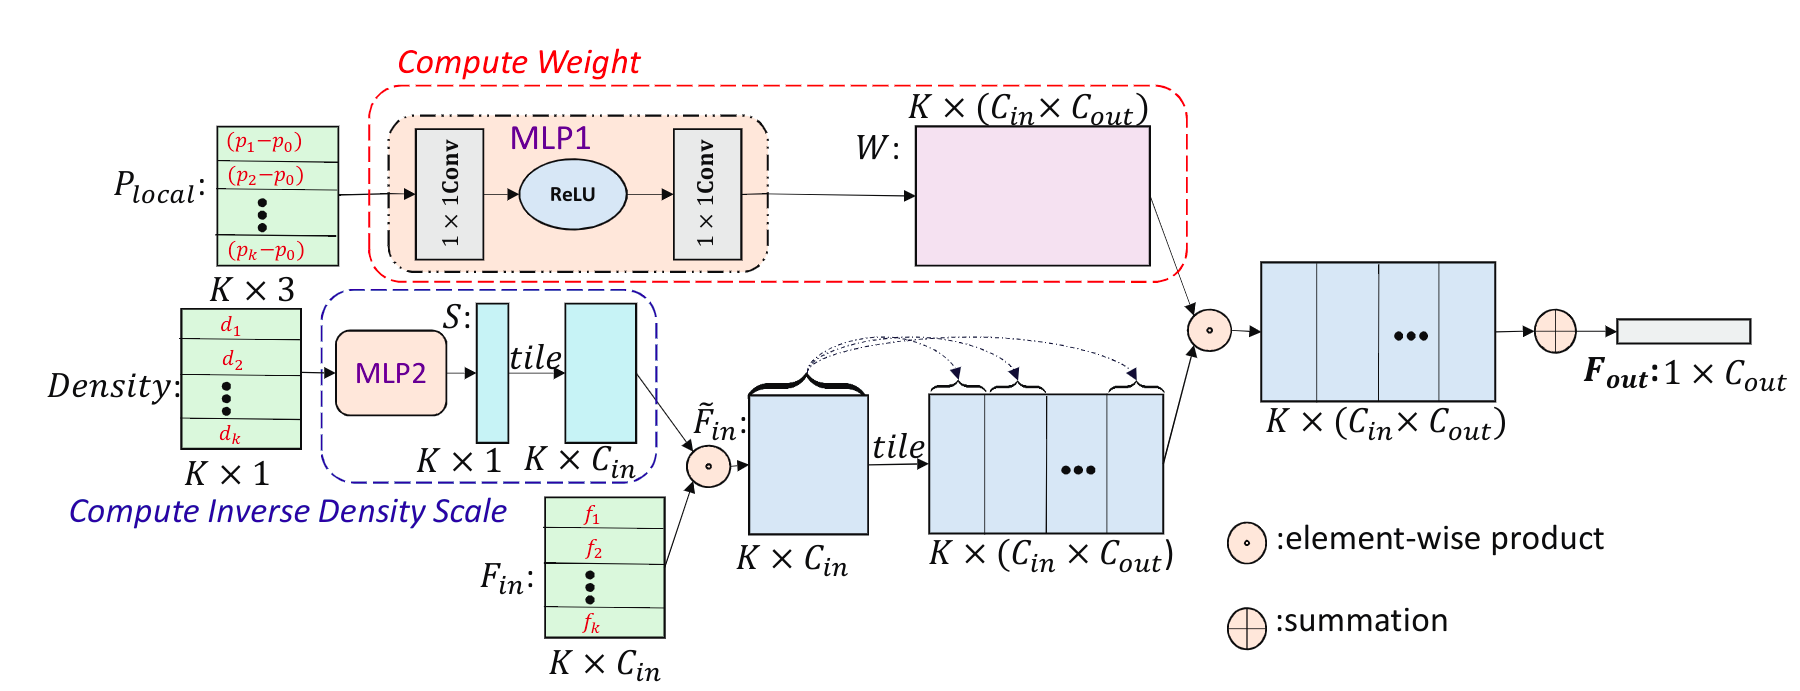
\includegraphics[width=\textwidth]{pointconv.png}
    \caption{PointConv operator~\cite{PointConv}}
    \label{fig:pointconvOperator}
\end{figure}

The weight function $W$ can be approximated by MLPs, while the density function, which outputs a value indicating how much points are concentrated around the centroid region, is calculated using kernel density estimation (KDE), described in~\cite{Turlach_bandwidthselection}, and then by appling a non-linear transform using an MLP.

The inputs of the PointConv operator are:

\begin{itemize}
    \item The subset of points $P_{local} \in \mathbb{R}^{K \times 3}$ : given a point $p_0$ in the point cloud, the $K$ closest points are taken and then the $p_0$ coordinates are subtracted to each point, obtaining the local coordinates of each point.
    \item The $ Density \in \mathbb{R} ^{K}$ estimated at each local point using KDE.
    \item The features $F_{in} \in \mathbb{R}^{K \times C_{in}}$, where $C_{in}$ is the number of channels, and for each channel there are the features associated with each local point. These features can be the point coordinates $(x, y, z)$, but also other features associated with the point such as the RGB color.
\end{itemize}

The \textit{Compute Weight} module is made by an MLP implemented as a $1 \times 1$ convolution, followed by a non-linear ReLU activation function, followed by another $1 \times 1$. The output of this module is $W \in \mathbb{R}^{K \times (C_{in} \times C_{out}})$.

The \textit{Compute Inverse Density Scale} module is used to calculate $S$: this is done by feeding the $Density$ into an MLP for a one dimensional linear transform. In this way the network can "decide" to use the density estimates.

Finally, the $F_{out} \in \mathbb{R}^{C_{out}}$ feature(s) associated with the feature(s) $F_{in}$ is:

\begin{equation}\label{eq:pointconv_orig}
\mathbf{F}_{\text {out }}=\sum_{k=1}^{K} \sum_{c_{i n}=1}^{C_{i n}} S(k) \mathbf{W}\left(k, c_{i n}\right) F_{i n}\left(k, c_{i n}\right)
\end{equation}

\paragraph{Architecture of a NN using PointConv} The architecture proposed in combination with PointConv is a hierarchical structure, composed by \textit{feature encoding blocks}. In each feature encoding block there is a sampling layer, a grouping layer and a PointConv. This feature encoding blocks (apart from the PointConv operator) are very similar to the ones already seen in PointNet++~\cite{qi2017pointnet++}, see also paragraph~\ref{par:pointnet++}. The only difference is that the neighbors of the centroid are calculated using the k-NN approach. In total the neural network is composed of 3 feature encoding blocks followed by 3 fully connected layers\footnote{See the code hosted on GitHub: \url{https://github.com/DylanWusee/pointconv_pytorch/blob/master/model/pointconv.py}}.

\paragraph{Efficient PointConv} A noticeable problem of the original PointConv operator is the memory needed for the $W$ function: given the batch size $B$, the number of points in the point cloud $N$, the number of local points $K$, the number of input channels $C_{in}$ and the number of output channels $C_{out}$ the size of the filter weight would be $B \times N \times K \times C_{in} \times C_{out}$.

It can be shown that PointConv equation~\ref{eq:pointconv_orig} can be reduced to a matrix multiplication and a 2D convolution. The new operator can be seen in figure~\ref{fig:efficientPointconv}. This can reduce the memory consumption by a factor of $1 / 64$.

\begin{figure}[ht]
    \centering
    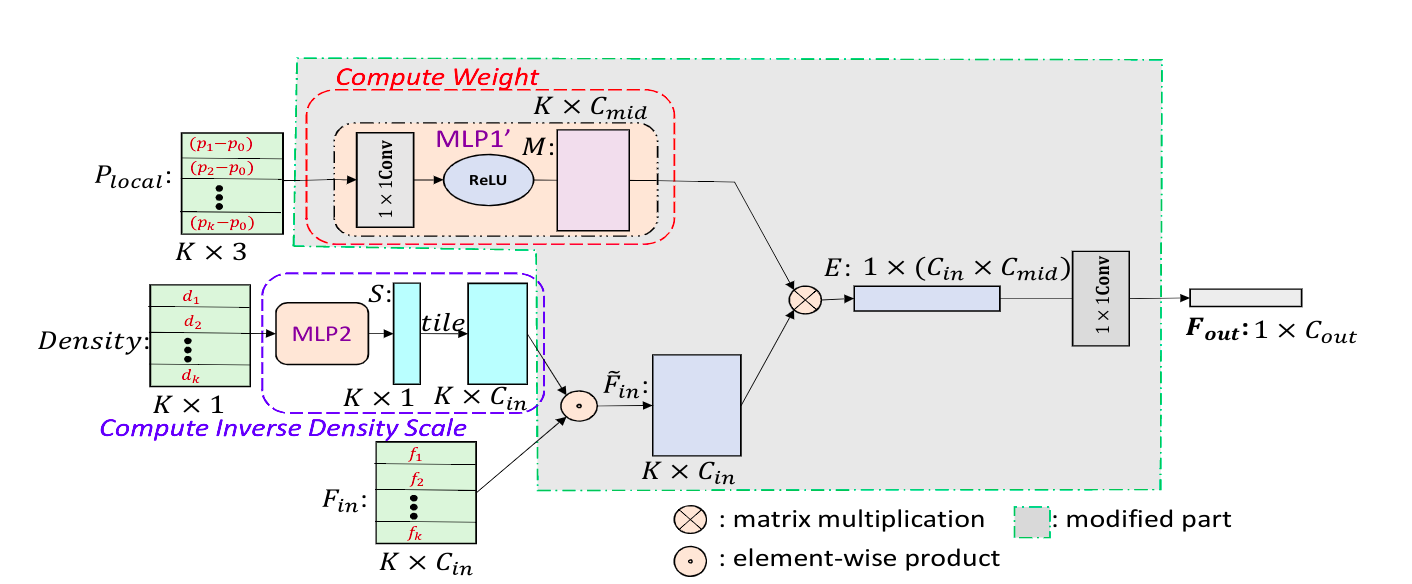
\includegraphics[width=\textwidth]{efficient_pointconv.png}
    \caption{Efficient PointConv~\cite{PointConv}}
    \label{fig:efficientPointconv}
\end{figure}

\paragraph{PointConv experiments}

The experiments have been performed on the ModelNet40 dataset, and have been conducted in the same way as PointNet authors did, which have become a standard to have a meaningful comparison between different networks. The overall accuracy obtained by PointConv on this dataset is $92.5$

An interesting experiment that has been carried out is the classification of CIFAR-10 dataset~\cite{Krizhevsky09learningmultiple}, which consists of 60000 32x32 colour images in 10 classes, with 6000 images per class. To demonstrate that PointConv is a good approximation of convolution the authors converted each point in an image into $(x,y)$ coordinates with the associated RGB color. Two CNNs have been trained, using PointConv as the convolution operator. The accuracy results in table~\ref{tab:pointconv_exp_cifar10} show that the networks using PointConv have roughly the same accuracy as normal CNNs, given that the overall architecture remains the same.

\begin{table}[ht]
    \centering
    \caption{CIFAR-10 experiments}
    \begin{tabular}{cc}
        \hline \text { Network } & \text { Accuracy (\%) } \\
        \hline AlexNet~\cite{AlexNet} & 89.00 \\
        VGG19~\cite{vgg19} & 93.60 \\
        \hline
        PointConv (5-layers) & 89.13 \\
        PointConv (VGG19) & 93.19 \\
        \hline
    \end{tabular}
    \label{tab:pointconv_exp_cifar10}
\end{table}

\subsubsection{Graph inspired networks}
As seen before, point clouds representations lack topological information.
An approach proposed by Wang et al.~\cite{Wang2019} involves constructing graphs associated with the point cloud, and then using a novel convolution operator, \textit{EdgeConv}.

\paragraph{EdgeConv} The edge convolution operates on a graph constructed from local regions of the point cloud.

Let $F$ be the feature number of each point in the point cloud. In the simplest case only the $(x,y,z)$ coordinates of the point are considered, so $F = 3$ but other features like RGB color can be used, for example if a 3D camera was employed to acquire the point cloud. In general $F$ is the dimensionality of the features in input to a layer.

To apply the edge convolution it must first be constructed a graph $G = (V,E)$, where $V \in \{1 \dots n\}$ are the vertices and $E \in V \times V$ are the edges. To construct a graph which represent a local structure in the point cloud a point is taken and then its $k$-nearest neighbors are computed. The graph will then have the points found as vertices and the connections between the point and its neighbors as edges.

An edge-feature is defined as $e_{ij} = h_{\Theta}(x_i, x_j) : R^F \times R^F \rightarrow R^{F'}$, where $h_{\Theta}$ is a non-linear function with $\Theta$ learnable parameters. The \textit{EdgeConv} operator is then defined by using an aggregation function $\square$ over the edge features associated with all the edges at each point. The output of EdgeConv at the vertex $x_i$ is:

\begin{equation}
\mathbf{x}_{i}^{\prime}=\underset{j:(i, j) \in \mathcal{E}}{\square} h_{\Theta}\left(\mathbf{x}_{i}, \mathbf{x}_{j}\right)
\end{equation}

After each EdgeConv layer the number of points in the point cloud remains the same, the input feature dimension is $F$ and the output feature dimension is $F'$.

\begin{figure}[ht]
    \centering
    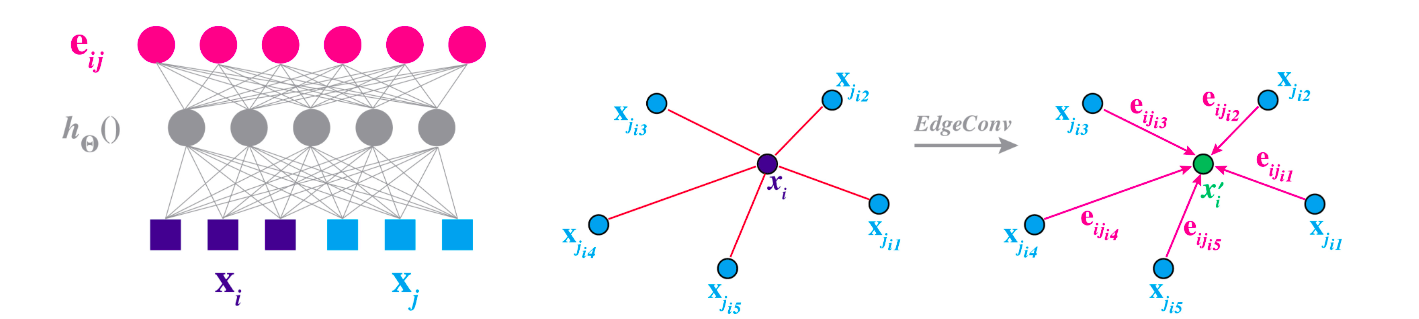
\includegraphics[width=\textwidth]{edgeconv.png}
    \caption{Left: the edge features $e_{ij}$, computed by a fully connected layer. Right: the edge features computed for each edge.~\cite{Wang2019}}
    \label{fig:edgeConvOperator}
\end{figure}

The choice of the $h_{\Theta}$ and $\square$ defines the properties of the EdgeConv operator. The authors of the paper chose an asymmetric edge function:

\begin{equation}\label{eq:edgeconv_h}
h_{\mathbf{\Theta}}\left(\mathbf{x}_{i}, \mathbf{x}_{j}\right)=\bar{h}_{\mathbf{\Theta}}\left(\mathbf{x}_{i}, \mathbf{x}_{j}-\mathbf{x}_{i}\right)
\end{equation}

This function takes into account both the global structure by using the coordinates of $x_i$ and the local structure by using the distances between $x_i$ and its neighbors. This function is easily implemented by an MLP.

As for the aggregation function $\square$ the authors chose the max function:

$$
x_{i}^{\prime}=\max _{j:(i, j) \in \mathcal{E}} e_{i j}^{\prime},
$$

The properties of the EdgeConv operator depend on the choice of the edge and aggregation functions.

Using the $\max$ aggregation achieves permutation invariance with respect to the order of the neighbor points $x_j$.

As for the translation invariance it can seen in equation~\ref{eq:edgeconv_h} that the operator is partially invariant on the translation. It is easy to demonstrate that $h_{\Theta}(x_i - x_j)$ is translation invariant, while $h_{\Theta}(x_i)$ isn't, as shown in equation~\ref{eq:edgeconv_tranls}.

\begin{equation}\label{eq:edgeconv_tranls}
\begin{split}
    \bar{h}_{\mathbf{\Theta}}\left((\mathbf{x}_{j} + T)-(\mathbf{x}_{i} + T), \mathbf{x}_{i} + T \right) = \\
    \theta \cdot ((\mathbf{x}_{j} + T)-(\mathbf{x}_{i} + T)) + \phi \cdot (\mathbf{x}_{i} + T) = \\
    \theta \cdot (\mathbf{x}_{j}-\mathbf{x}_{i}) + \phi \cdot (\mathbf{x}_{i} + T)
\end{split}
\end{equation}


If only the first part is considered then EdgeConv is fully invariant to translation, however the global structure information would be lost: the classification would be based on patches of the point cloud without taking into account the global pose of these patches.

\paragraph{Dynamic graph update}
An important part explored is the dynamic graph computation.
State of the art approaches in graph based network compute the graph at the beginning and then use it throughout the network. DGCNN instead recomputes the graph after each EdgeConv layer: the architecture learns how to construct the graph.
The k-nearest neighbors are found by computing the pairwise distance matrix in feature space.

\paragraph{Architecture and results}

The network architecture used for the evaluation experiments is shown in figure~\ref{fig:DGCNN}. It is composed of 4 EdgeConv layers with skip connections to aggregate multi scale features, obtaining a 512-dimesional point cloud, and a max pooling layer. Then there are multiple fully connected layers. All layers include leaky ReLU as activation function and batch normalization.

\begin{figure}[ht]
    \centering
    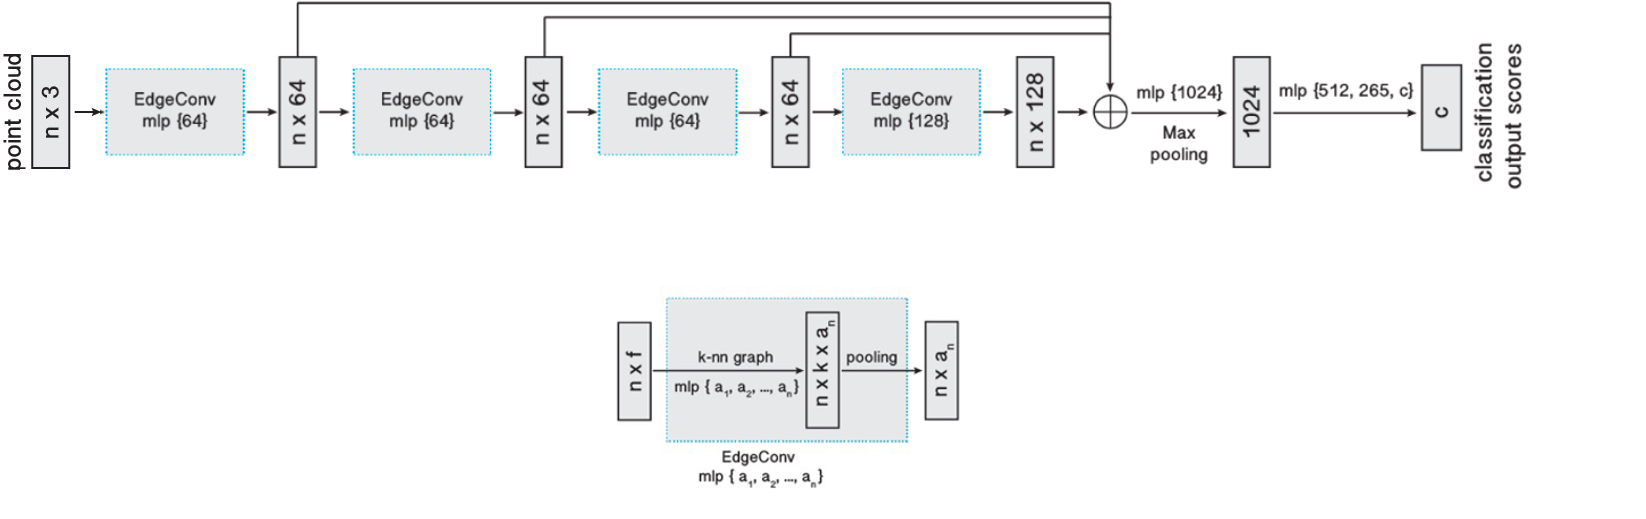
\includegraphics[width=\textwidth]{DGCNN_orig.png}
    \caption{Top: DGCNN network architecture. Bottom: EdgeConv.~\cite{Wang2019}}
    \label{fig:DGCNN}
\end{figure}

The experiments have been performed on ModelNet40, and have been conducted in the same way as PointNet authors did, which have become a standard to have a meaningful comparison between different networks.

The baseline model uses only a fixed graph (no dynamic computation), and uses as edge function $ h_{\Theta}(x_i, x_j)$. With this model an improvement of $\SI{1}{\percent}$ over PointNet++ is achieved.

Multiple experiments have been performed to evaluate how much each part of the model influences the accuracy results, as shown in table~\ref{tab:dgcnn_exp}.
Three improvements to the networks have been tried:

\begin{itemize}
    \item Centralization, which is using explicitly the global information given by the vertex $x_i$ and the distance between its neighbors, by using the edge function ${h}_{\mathbf{\Theta}}\left(\mathbf{x}_{i}, \mathbf{x}_{j}-\mathbf{x}_{i}\right)$.
    \item Dynamic graphs, which is the computation of the neighbors on the features extracted for each EdgeConv layer.
    \item More points, by using 2048 points instead of 1024.
\end{itemize}

\begin{table}[htb]
    \centering
    \caption{CENT denotes centralization, DYN denotes dynamical graph recomputation and MPOINTS denotes experiments with 2,048 points}
    \begin{tabular}{ccccc}
        \hline \text { CENT } & \text { DYN } & \text { MPOINTS } & \text { MEAN CLASS ACCURACY(\%) } & \text { OVERALL ACCURACY(\%) } \\
        \hline x & & & 88.9 & 91.7 \\
        x & x & & 89.3 & 92.2 \\
        x & x & x & 90.2 & 92.9 \\
        \hline
    \end{tabular}
    \label{tab:dgcnn_exp}
\end{table}

It is also worth noticing that DGCNN performs faster than state of the art network such as PointNet++, while keeping the model size relatively small, as shown in table~\ref{tab:dgcnn_exp2}.

\begin{table}[htb]
    \centering
    \caption{Size and time comparison between PointNet, PointNet++ and DGCNN }
    \begin{tabular}{lccc}
        \hline & \text { MODEL SIZE(MB) } & \text { TIME(MS) }  \\
        \hline \text { POINTNET (BASELINE) (QI ET AL. 2017B) } & 9.4 & 6.8  \\
        \text { POINTNET (QI ET AL. 2017B) } & 40 & 16.6 \\
        \text { POINTNET++ (QI ET AL. 2017C) } & 12 & 163.2 \\
        \text { DGCNN (BASELINE) } & 11 & 19.7  \\
        \text { DGCNN } & 21 & 27.2  \\
        \hline
    \end{tabular}
    \label{tab:dgcnn_exp2}
\end{table}

\section{Comparison}\label{sec:comparison}
In this survey we have investigated the main point cloud classification approaches: projection-based and point-based. Projection-based approaches transform the unstructured 3D point clouds into specific modality, such as multi-view, voxels or pillars, and extract features from the target format. Point-based approach, on the other side, learn features directly from the points and not from their spatial arrangement.

As examples of projection-based approaches, we've described the multi-view and the volumetric methods; in the former the information in multiple 2D views of an object is compiled in a compact descriptor with a CNN, in the latter the cloud points are projected into volumetric occupancy grids on which a CNN performs the classification task. As examples of the multi-view method we have the CNNs \textit{FV 12x} and \textit{MVCNN}, while the volumetric approach is represented by \textit{VoxNet}.

In the context of point-based approach, the three main methods are MLP, where features from every point are extracted with independent multi-layer perceptrons, CNN, networks that are directly fed with points and define a special type of convolution, and graph inspired networks, that exploit the topological information already present in the point cloud. As representants of these three methods we have respectively PointNet and PointNet++ as MLPs, PointConv as as CNN and EdgeConv as a graph inspired network.

% TODO: vorrei aggiungere un confornto tra i vari metodi che usano le reti per ottenere permutation invariance e translation/rotation invariance.
% TODO le cose che sto scrivendo per questa parte sono da guardare un attimo insieme, ho scritto quello che ho vagamente interpretato dalle sezioni sopra ma non ho letto i paper

\paragraph{Permutation invariance} Permutation invariance allows the network to not being sensitive to the order of the points in the point cloud.

Projection based methods do not need an explicit way to handle the permutation of the points in the point cloud, since the points get projected either on images or voxels before being fed to the network. The methods used to project the points are invariant to the permutations of the point cloud.

Point based methods seen in this survey have different ways to achieve this property:

\begin{itemize}
    \item PointNet and PointNet++ TODO
    \item PointConv uses the same MLP weights for each point in the PointConv layer. TODO non sono convinta
    \item DGCNN uses a symmetric aggregation function (the authors used the max function).
\end{itemize}

\paragraph{Transformation invariance} Transformation invariance allows the network to be robust to geometric transformations such as rotation and translation.

Projection based methods TODO

Point based methods TODO

\paragraph{Results comparison}

The only dataset on which all neural networks have been tested is ModelNet40.

In table \ref{tab:comparison_results} the overall accuracy results are shown.

\begin{table}[H]
    \centering
    \begin{tabular}{lccc}
        \hline & \text { MODEL SIZE(MB) } & \text { TIME(MS) } & \text { ACCURACY(\%) } \\
        \hline 
        \text { FV 12x} & - & - & 84.8 \\
        \text { MVCNN} & - & - & 90.1 \\
        \text { VoxNet} & - & - & 83.0 \\
        \text { POINTNET (QI ET AL. 2017B) } & 40 & 16.6 & 89.2 \\
        \text { POINTNET++ (QI ET AL. 2017C) } & 12 & 163.2 & 91.9 \\
        \text { PointConv} & 11 & 19.7 & 92.5 \\
        \text { DCG } & 21 & 27.2 & 92.9 \\
        \hline
    \end{tabular}
    \caption{Results for each network, tested on ModelNet40}
    \label{tab:comparison_results}
\end{table}

vedi table 2 di guo2020

vedi supplementary B del paper di pointnet per comparazione tra pointnet e voxnet (con grafico!)

\section{Conclusion}
TODO inventare qualcosa

In this survey, a short list of point cloud classification networks was made, highlighting the different approaches seen in literature.

Different networks use different methods to achieve the same properties needed for treating point clouds: permutation invariance and transformation invariance.


The neural networks described and the classification task tested on an easy, synthetic dataset might seem not really useful in real case applications. Instead, it is worth noting that the methods here described have paved the way of the more difficult tasks described in section \ref{sec:intro}.
For example we can see from the survey by Zhang et al \cite{ZHANG2020222} some neural networks that do point cloud registration are based on the methods described above: PointNetLK \cite{pointnetlk} is based on PointNet, DeepVCP \cite{deepvcp} is based on PointNet++, DCP\cite{dcp} is based on DGCNN.

\bibliographystyle{unsrt}  

\bibliography{references}

\end{document}
